\documentclass[a4paper,utf8]{article}
\usepackage[heading,fancyhdr]{ctex}
\usepackage{amsmath,amssymb,geometry,lastpage,ulem}
\usepackage{array,tabularx,tabulary,mhchem,xspace}
\usepackage{floatrow,subfig,multirow,bigstrut}
\usepackage{siunitx,booktabs,longtable,graphicx,xfrac,nameref}
\lineskiplimit=1pt
\lineskip=3pt
\geometry{
    top=25.4mm, 
    left=25mm, 
    right=25mm, 
    bottom=25mm,
    headsep=5.9mm,
}
\ctexset{
    section = {format+=\raggedright}
}
\newcommand{\fgref}[1]{图~\ref{#1}\xspace}
\newcommand{\seqref}[1]{式~(\ref{#1})}
\newcommand{\expinfo}[7][无]{
    {\zihao{-3}\bfseries\songti
    实验名称:\uline{\hfill\mbox{#2}\hfill} \\[2.9mm]
    学\quad 号:\uline{\makebox[25mm]{#3}}\hfill
    姓\quad 名:\uline{\makebox[25mm]{#4}}\hfill
    班\quad 级:\uline{\makebox[25mm]{#5}} \\[2.9mm]
    合作者:\uline{\makebox[25mm]{#1}} \hfill
    桌\quad 号:\uline{\makebox[25mm]{#6}}\hfill\makebox[25mm+4em]{}\\[2.9mm]
    实验日期:\uline{\makebox[30mm]{#7}}\hfill\mbox{} \\[58.7mm]
    }
}
\newcommand{\pointingbox}{
    {\zihao{4}\bfseries\songti%
    实验考核\\[3mm]
    \extrarowheight=3mm
    \begin{tabularx}{150mm}{|X|X|X|X|X|}\hline
        \hfil 项目 \hfil  & \hfil 实验预习 \hfil & \hfil 实验过程 \hfil & \hfil 分析与讨论 \hfil & \hfil 总评 \hfil \\[3mm] \hline
        \hfil 评价 \hfil &  &  &  &  \\[3mm] \hline
    \end{tabularx}
    }
}
\newcommand{\derivative}[2]{\frac{\mathrm{d} #1}{\mathrm{d} #2}}
\newcommand{\thinking}[2]{\textbf{#1}\\
答:\begin{minipage}[t]{0.85\textwidth}
    #2
\end{minipage}}
\pagestyle{fancy}
\fancyhf{} \fancyhead[C]{电路基础实验} \fancyfoot[C]{\thepage~/~\pageref{LastPage}}
\newcounter{Rownumber}
\newcommand*{\Rown}{\stepcounter{Rownumber}\theRownumber}
\newcommand*{\resetRown}{\setcounter{Rownumber}{0}}
\newcommand{\qrange}[3]{\qtyrange[range-phrase = \text{$\sim$},range-units =single]{#1}{#2}{#3}}
\floatsetup[table]{capposition=top}
\newcolumntype{C}{>{\hfil}X<{\hfil}}
\renewcommand{\Nameref}[1]{\textbf{\ref{#1}~\nameref{#1}}} %导入导言

\begin{document}
\begin{center}
    {\mbox{}\\[7em]\zihao{2}\bfseries\songti%
    电路基础实验报告}\\[34mm]
    \expinfo[张泽钒]{二阶电路动态过程的研究}{22301077}{张蕴东}{22 高分子}{35}{2024.6.11}
\end{center}
\newpage

\section{实验目的}
\begin{enumerate}
    \item 研究二阶电路动态过程的零状态响应和零输入响应的基本规律和特点。
    \item 分析电路参数 R、L、C 对二阶电路动态过程响应的影响。
    \item 学习使用双线示波器观察动态过程波形的方法。
    \item 学习方波信号源的使用方法。
\end{enumerate}

\section{实验原理}%简单描述,含必要的公式和附图;
\begin{itemize}
    \item 二阶线性电路。从电路原理我们知道,用二阶线性常微分方程来描述的电路称为二阶线性电路。本实验研究有一个电感和电阻,又有一个电容的二阶电路,在方波激励时响应的动态过程
    \item 对于 RLC 串联的二阶电路,无论是零状态响应,还是零输入响应,电路过渡过程中性质完全由特征方程上 $LC_P^2+RC_P+1=0$ 的特征根 $P_1$,$P_2$来决定。$$\mathrm{P}_{1,2}=-\frac{\mathrm{R}}{2\mathrm{L}}\pm\sqrt{(\frac{\mathrm{R}}{2\mathrm{L}})^2-(\frac{1}{\sqrt{\mathrm{LC}}})^2}=-\delta\pm\sqrt{\delta^2-\omega_0^2}$$
    从上式可看出,特征根 $P_1$,$P_2$ 实际由电路 R、L、C 三个元件参数的数值大小来决定:如果 $R>2\sqrt{L/C}$,电路动态过程的性质为过阻尼的非振荡的过程;如果 $R=2\sqrt{L/C}$,电路动态过程的性质为临界阻尼过程;如果 $R<2\sqrt{L/C}$,电路动态过程的性质为欠阻尼的衰减振荡;如果 $R=0$,电路动态过程为等幅振荡;如果 $R<0$,电路动态过程为增幅振荡;\par
    从上述可知,通过改变电路的参数电阻 R(含负阻)、电感 L 或电容 C 的值,均可使电路发生上述几种不同性质的过渡过程。为研究二阶电路动态过程的性质,实际单元板上电路参数 R、L、C 各给出 $2 \sim 3$ 个值
    \item 动态过程性质的观察、测量与激励源频率(周期)的选择。动态过程很快,只能用示波器进行观察。用示波器观察必须使动态过程周期地重复出现。为了达此目的,本实验激励采用频率( $15\unit{\Hz} \sim 1.5\unit{\kHz}$)可调的方波信号源。它对电路的作用可以这样来理解,在方波电压大于 0 的正半个周期,输入电压由零跳变为 u0,使电路突然与一个直流电压 u0接通,相当于电路的零状态响应;方波后半个周期,输入电压又由 u0跳变为 0,使电路输入端突然短路,相当于电路的零输入响应。通过调方波电源频率而改变方波电压的周期使其半周期的时间远远大于过渡过程持续时间时(一般可选方波信号源的半周期和电路谐振时的周期保持 5:1 左右),就可由示波器观察到动态过程的全过程(包括零输入响应和零状态响应)。
    
    \item 实验方法说明。观察动态过程可采用电感、电容参数一定时调电阻的方法,也可采用电阻一定调电感、电容的方法。用示波器观察时,采用电源频率不变,电感、电容不变,只调电阻;或者采用电感、电容和电阻一定,调电源频率的方法。但无论如何调,心中要有数,不然调来调去什么现象都观察不到。
\end{itemize}

\section{实验仪表}
    实验电路见电路原理实验箱《二阶电路动态过程的研究》单元,$R_w=0 \sim 1\unit{\kilo\ohm}$、$R2= 10\unit{\ohm}$、$C1= 0.1\unit{\uF}$、$C2= 0.22\unit{\uF}$、$C3= 0.047\unit{\uF}$、$L1= 5\unit{\mH}$、$L2= 10\unit{\mH}$。

\section{实验内容与结果}
    \subsection{测试准备}
    \subsection{RLC 电路动态过程的测试与观察}

\section{实验结果}
    \subsection{过程记录汇总}
    由于本次实验测到的图比较重复,这里选取了一个效果较好条件作为代表进行展示和分析:\par
    电路参数:$L= 5\unit{\mH}$,$C= 0.1\unit{\uF}$
    \newpage
        \begin{figure}[!ht]
            \subfloat[$U_0$]{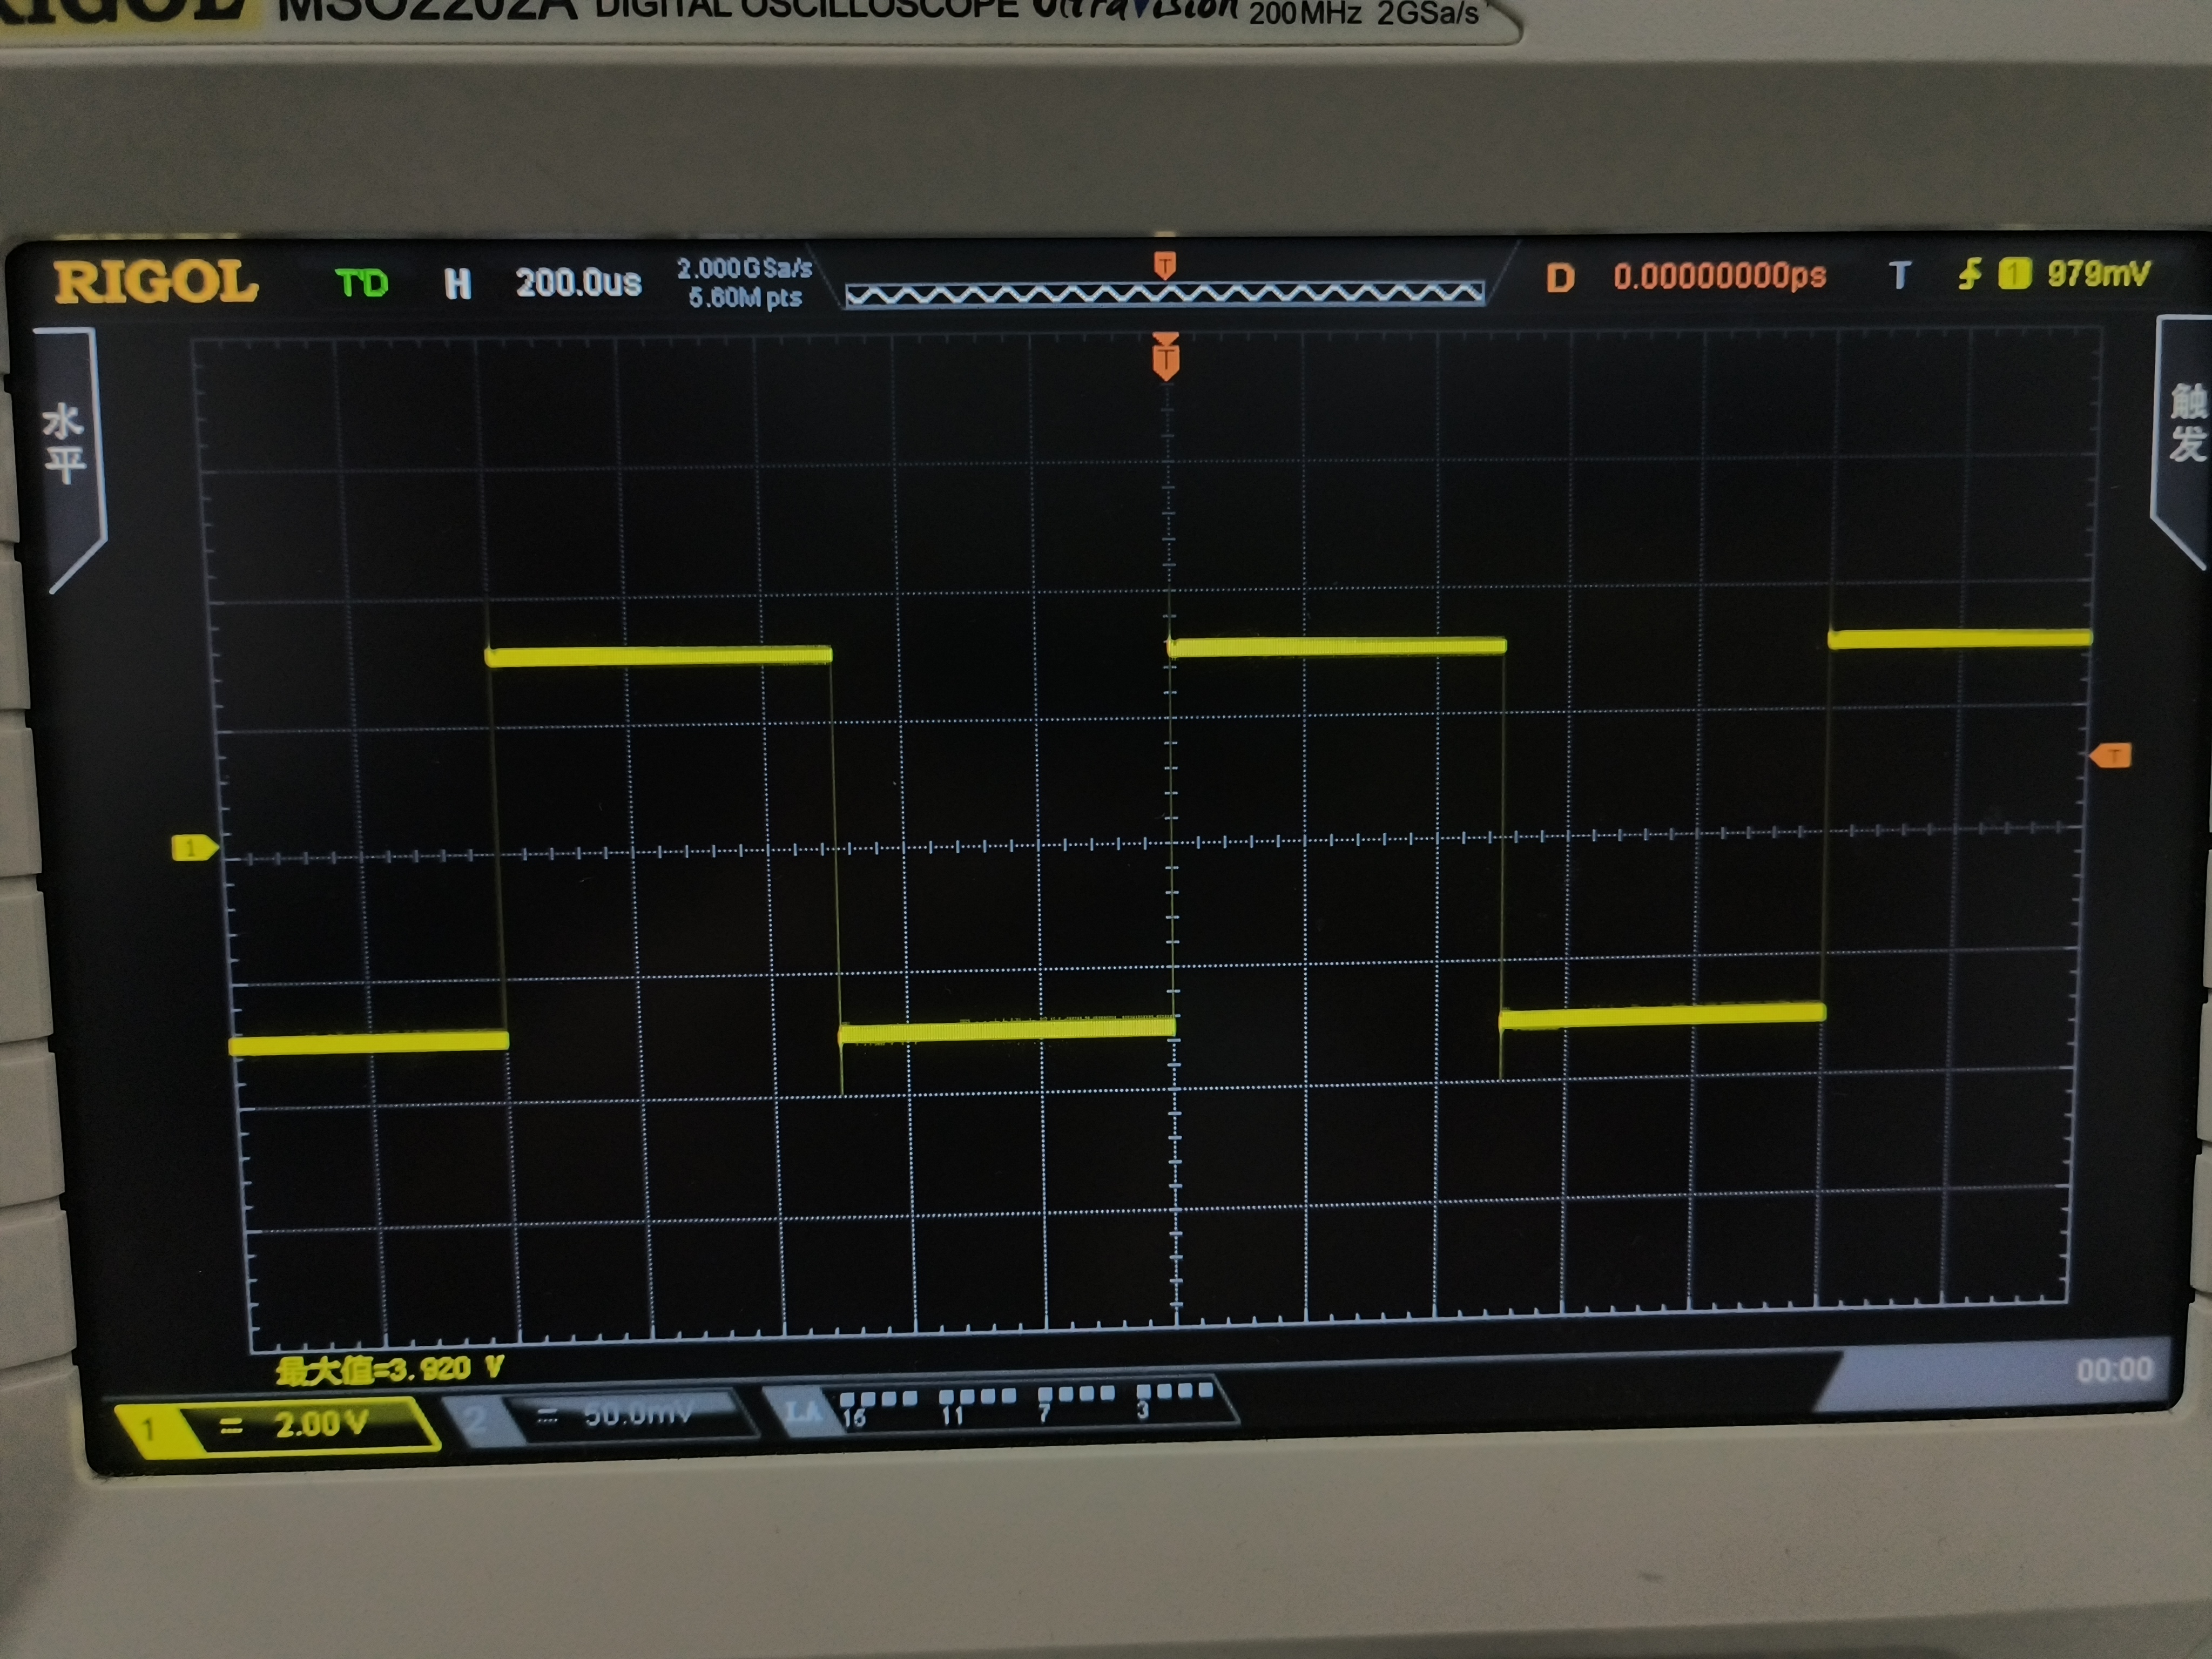
\includegraphics[width=0.43\textwidth]{sq.jpg}}\hspace{6mm}
            \subfloat[$U_C$]{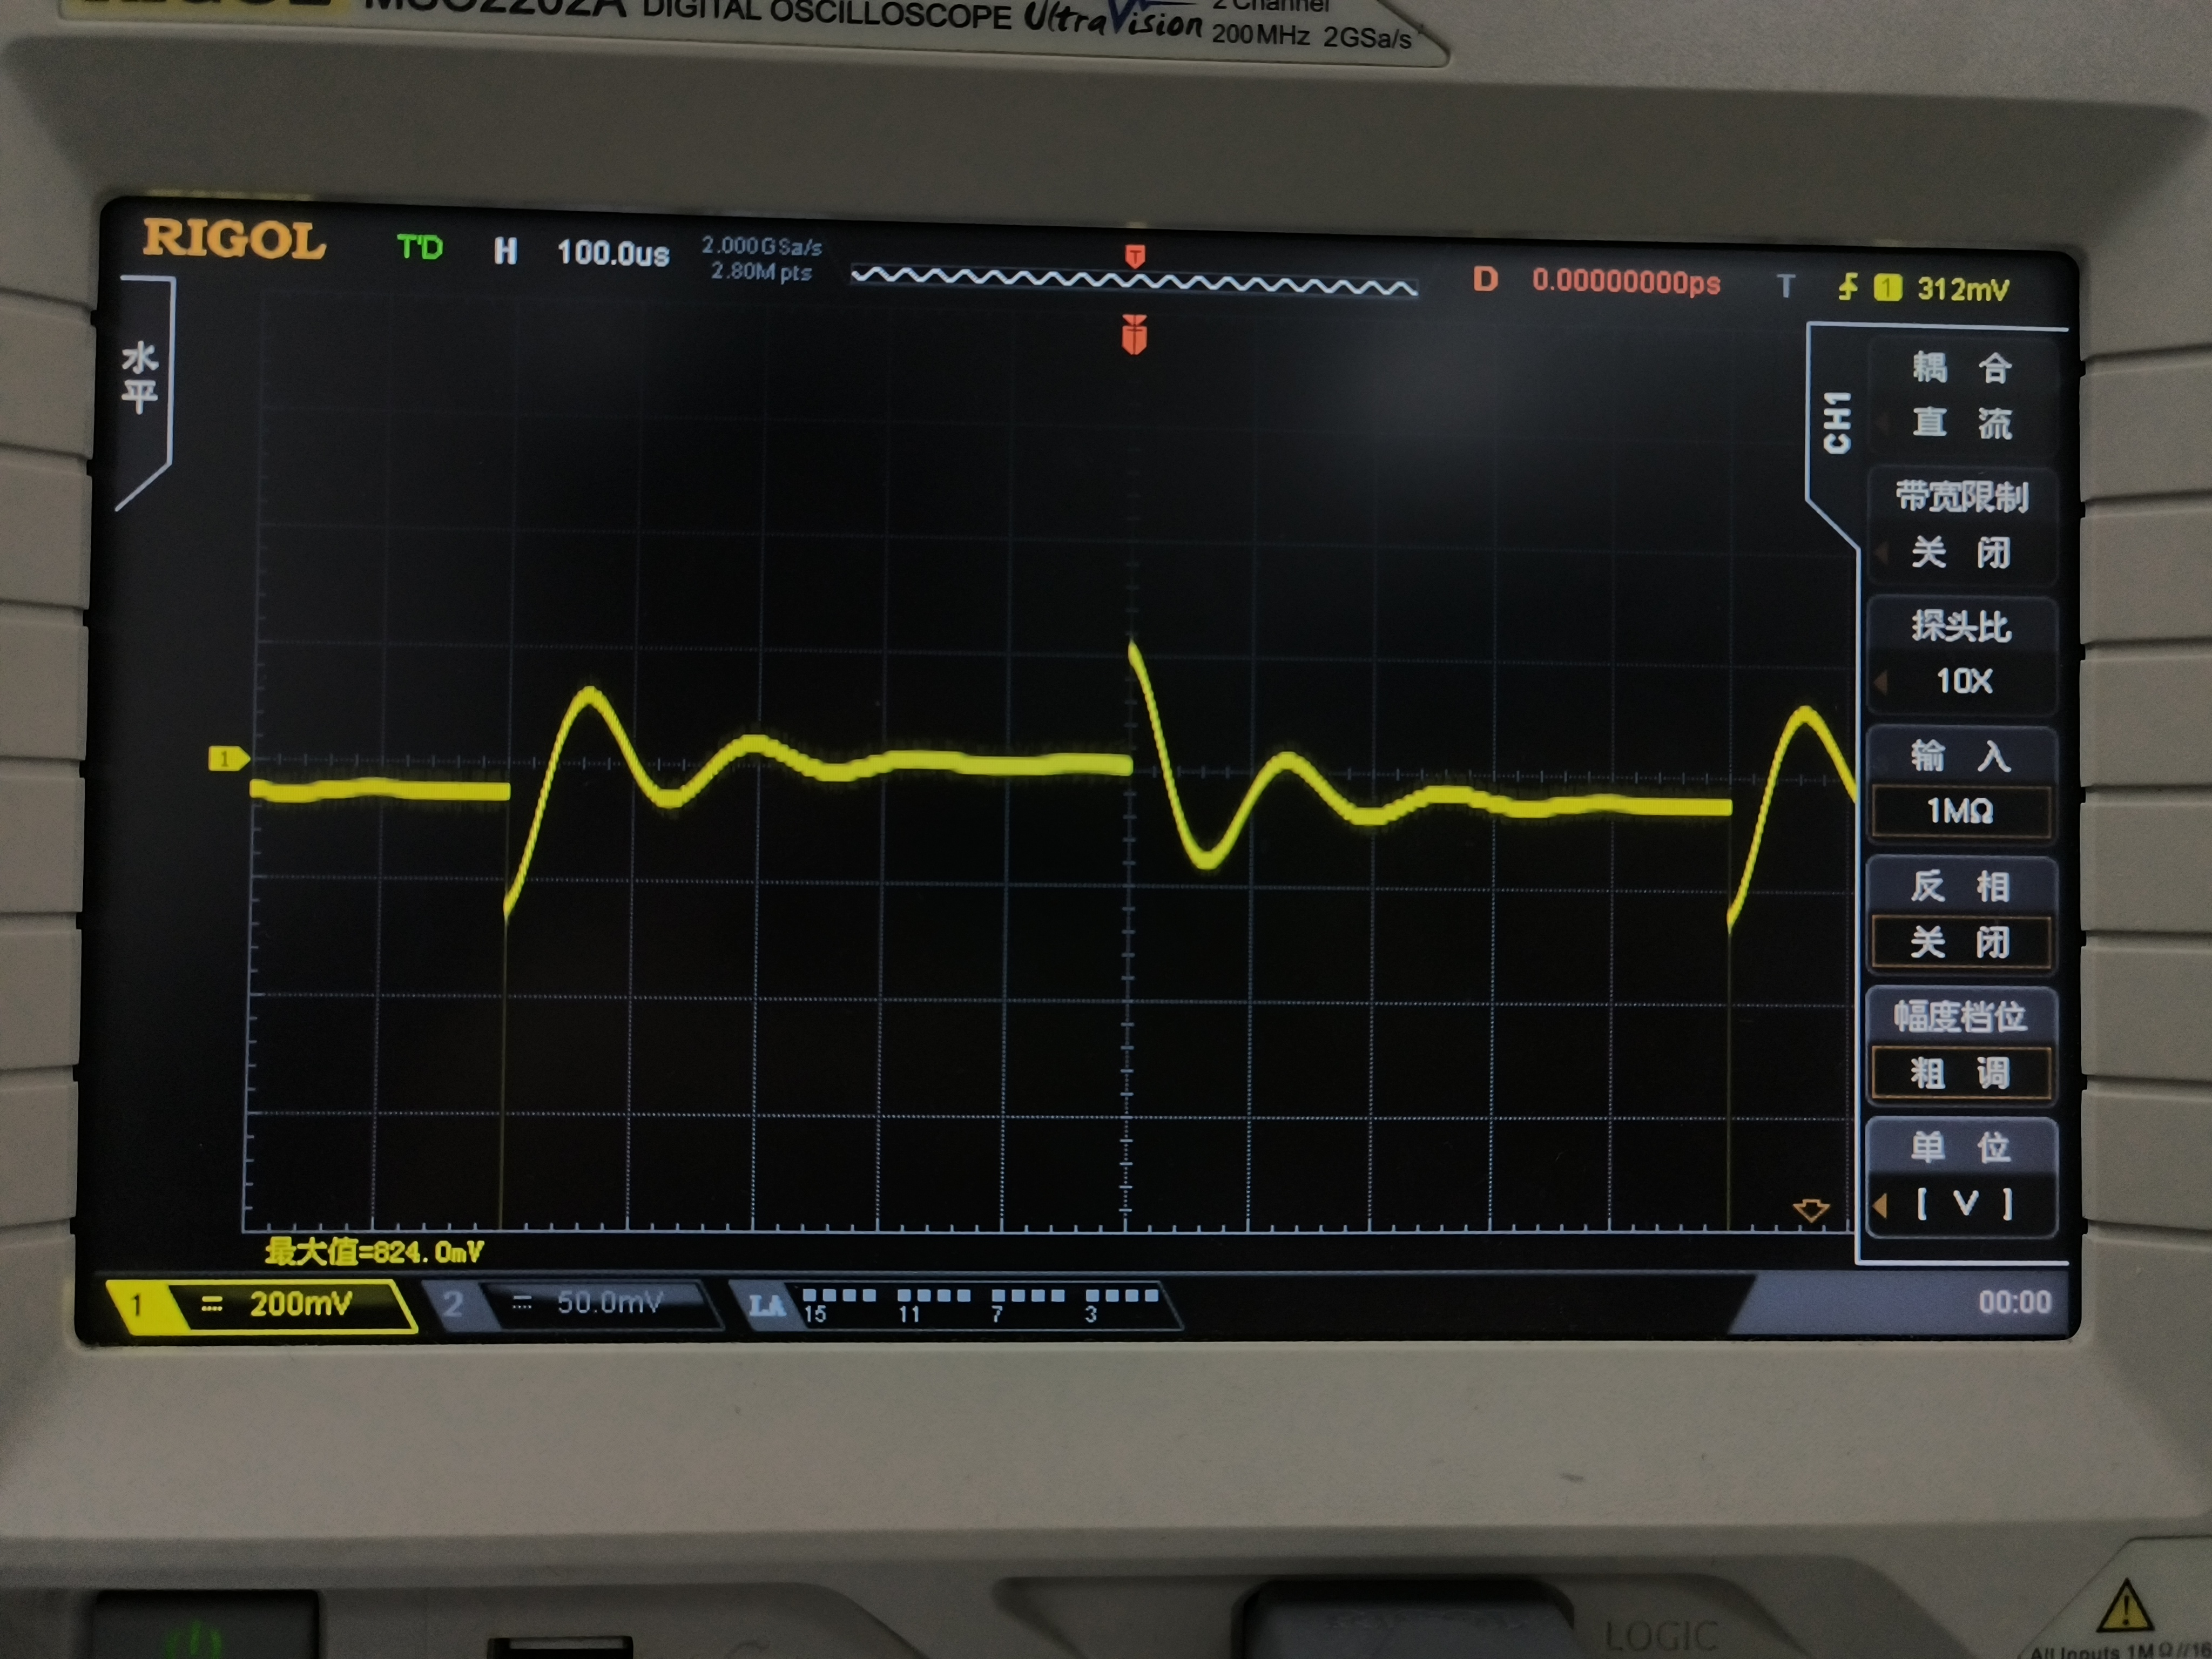
\includegraphics[width=0.43\textwidth]{1b.jpg}}\\
            \subfloat[$U_L$]{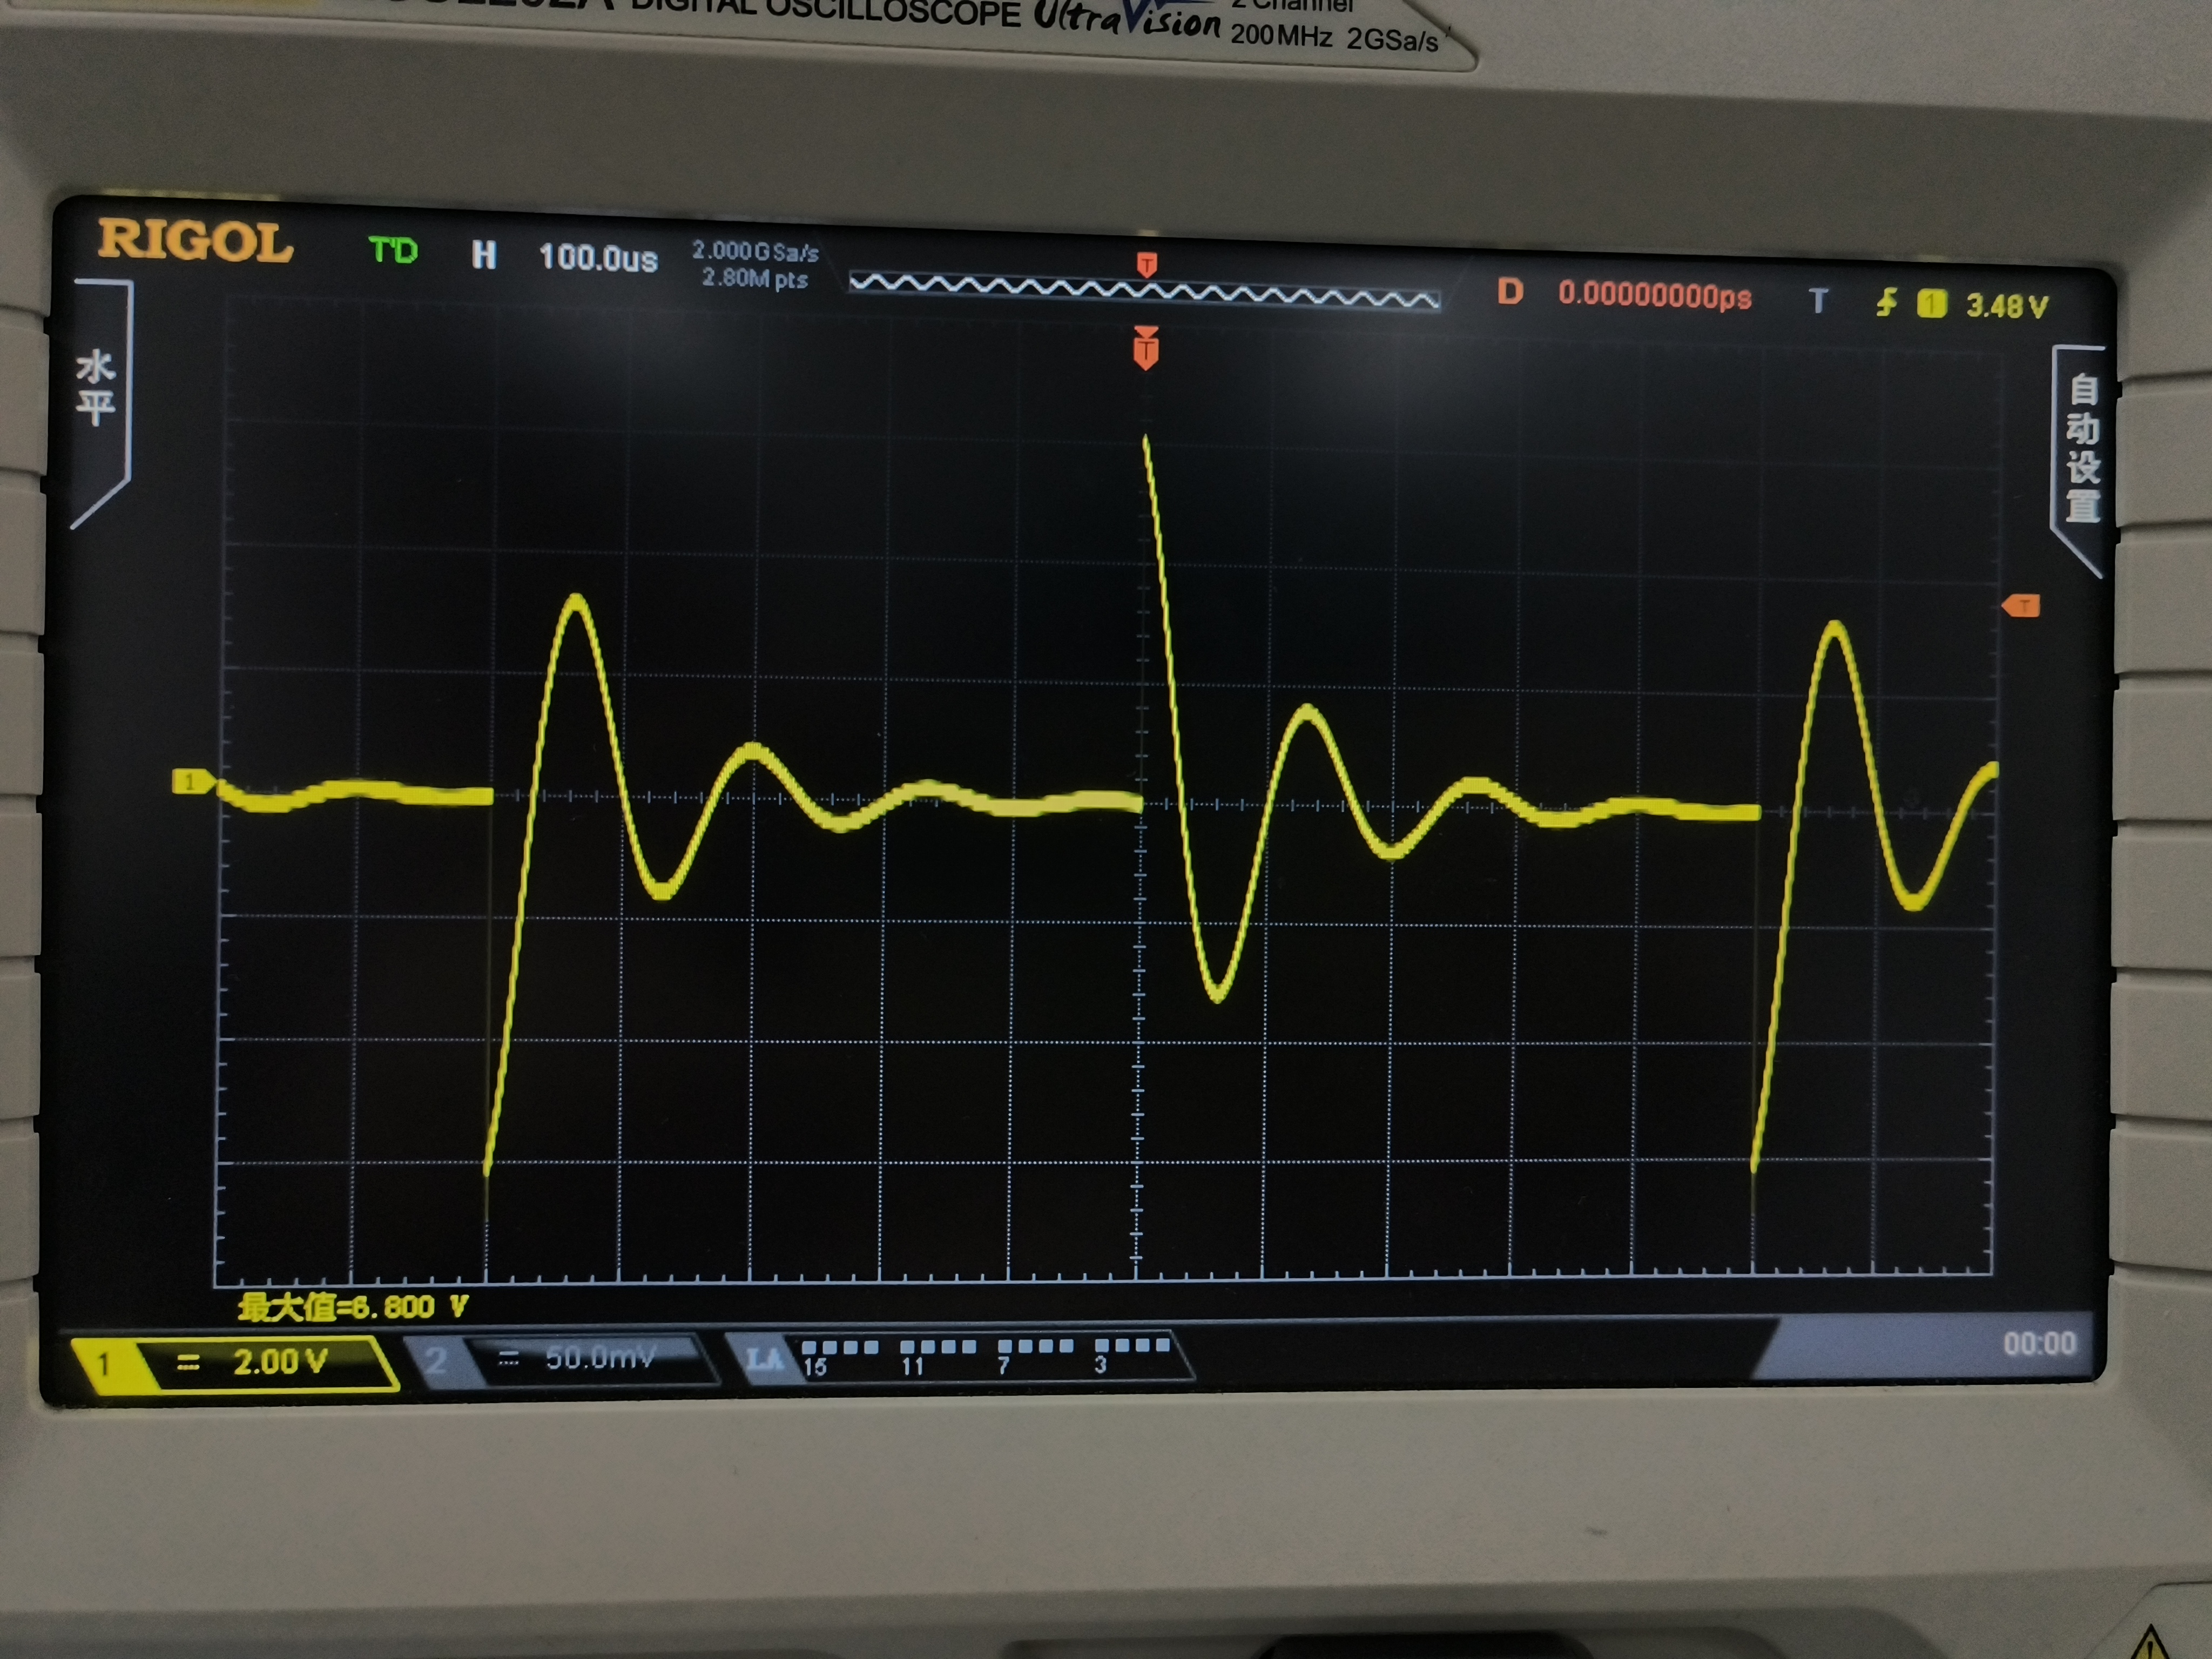
\includegraphics[width=0.43\textwidth]{1c.jpg}}\hspace{6mm}
            \subfloat[$U_R$]{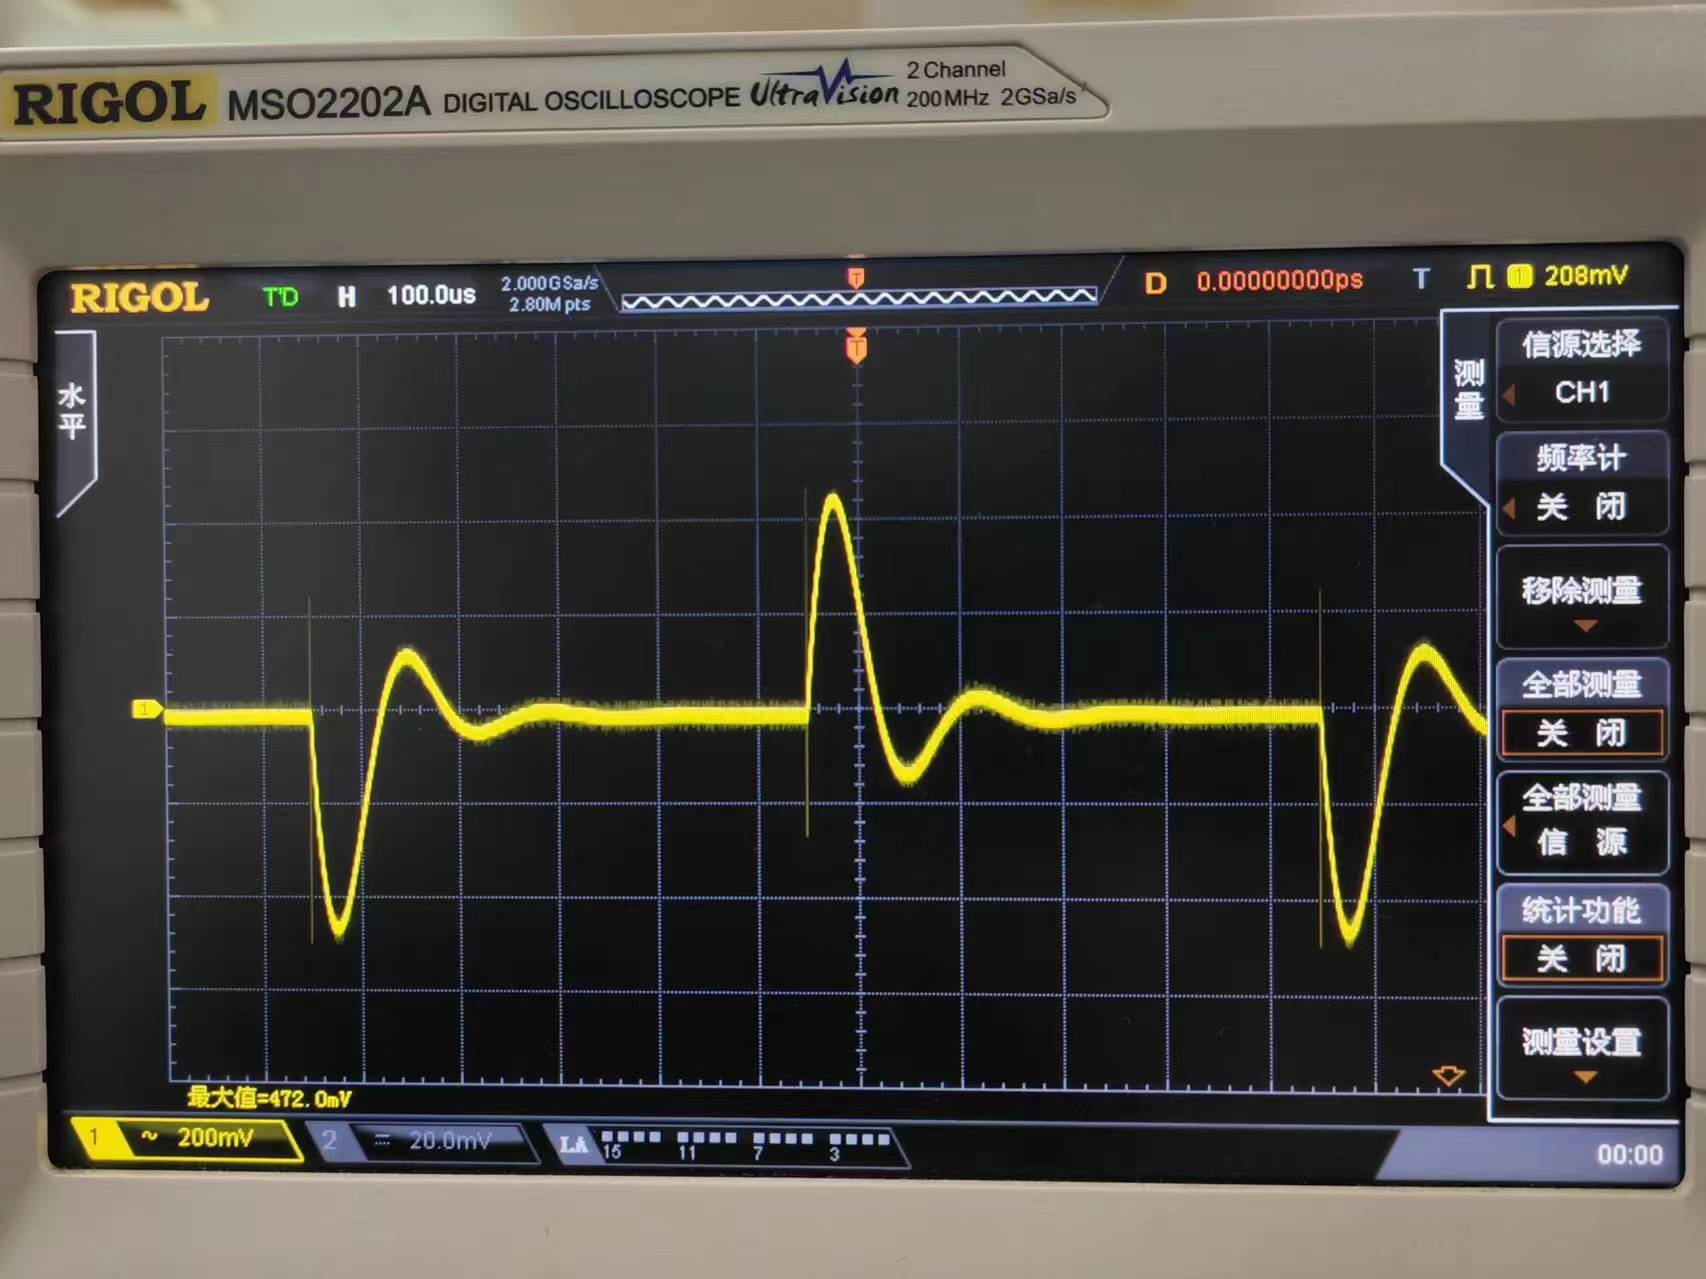
\includegraphics[width=0.43\textwidth]{1d.jpg}}
            \caption{$R=51\unit{\ohm}$(欠阻尼)}
        \end{figure}\par
        ~
        \begin{figure}[!ht]
            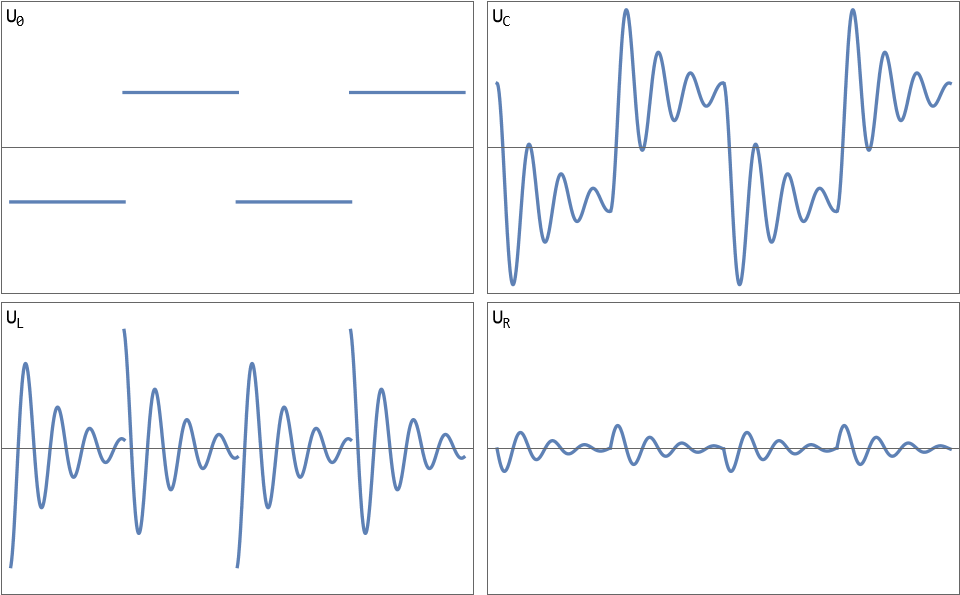
\includegraphics[width=0.9\textwidth]{1e.png}
            \caption{理论计算结果}
        \end{figure}\par

        \begin{figure}[!ht]
            \subfloat[$U_0$]{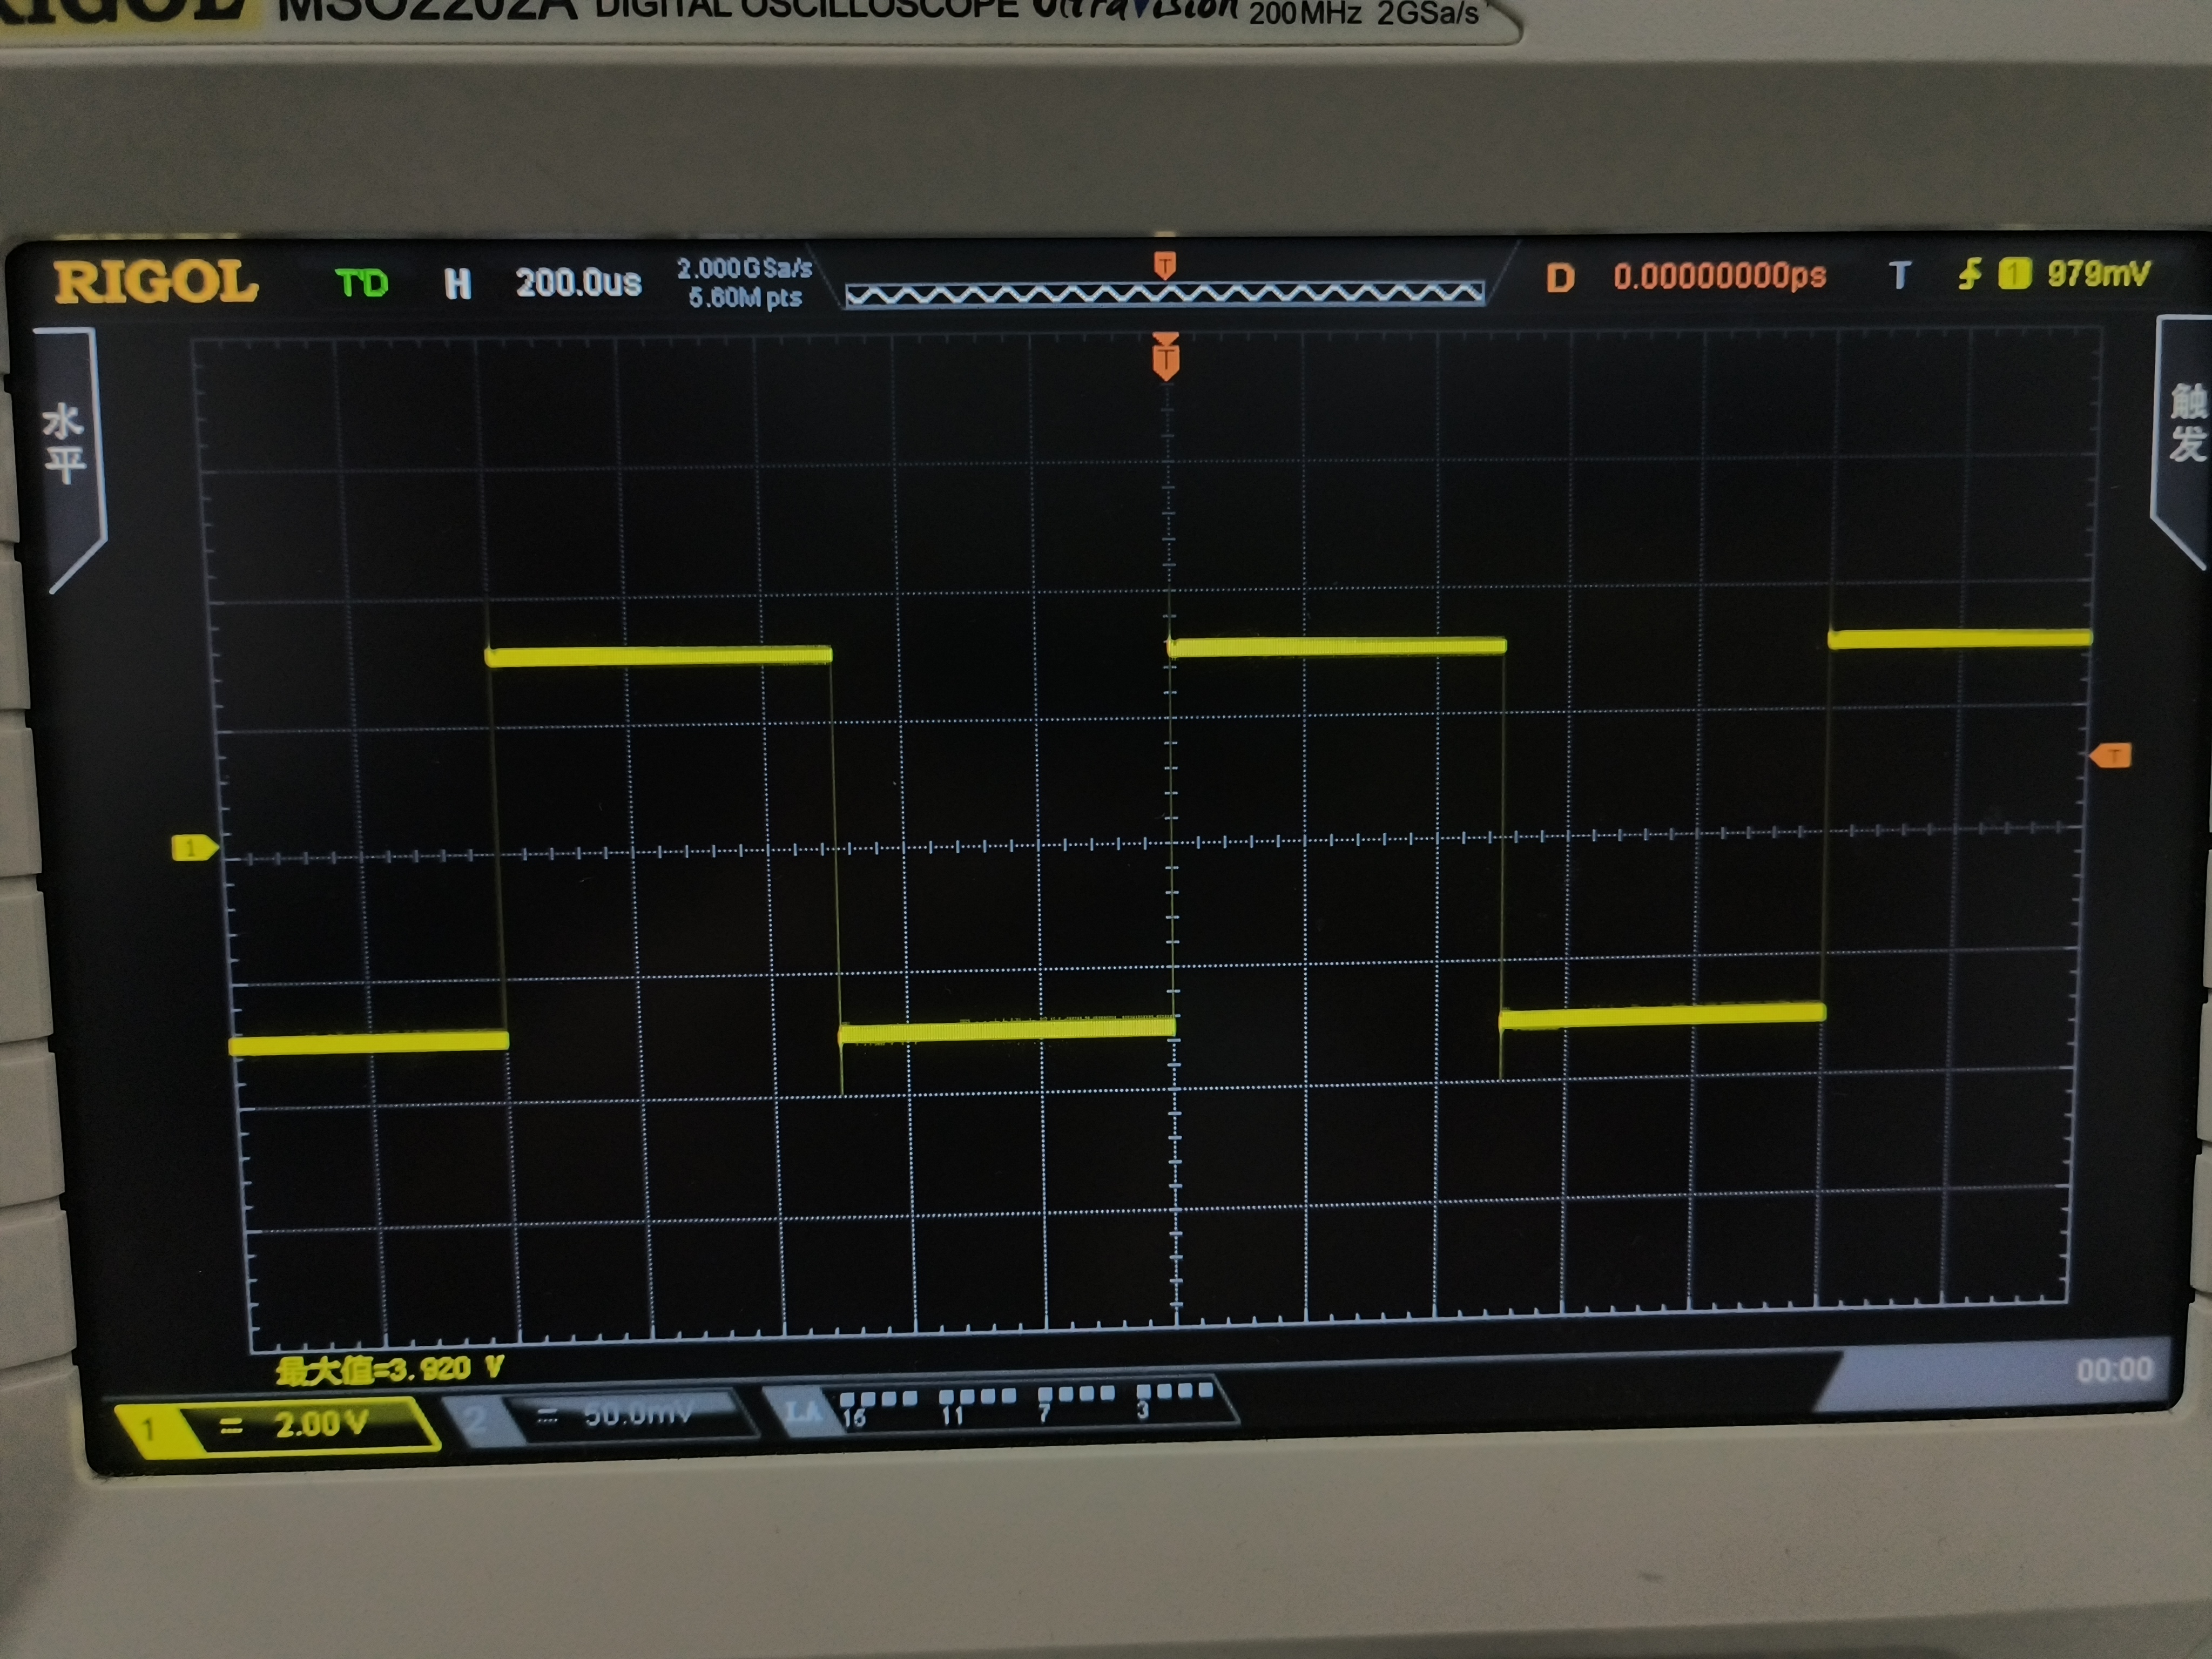
\includegraphics[width=0.43\textwidth]{sq.jpg}}\hspace{6mm}
            \subfloat[$U_C$]{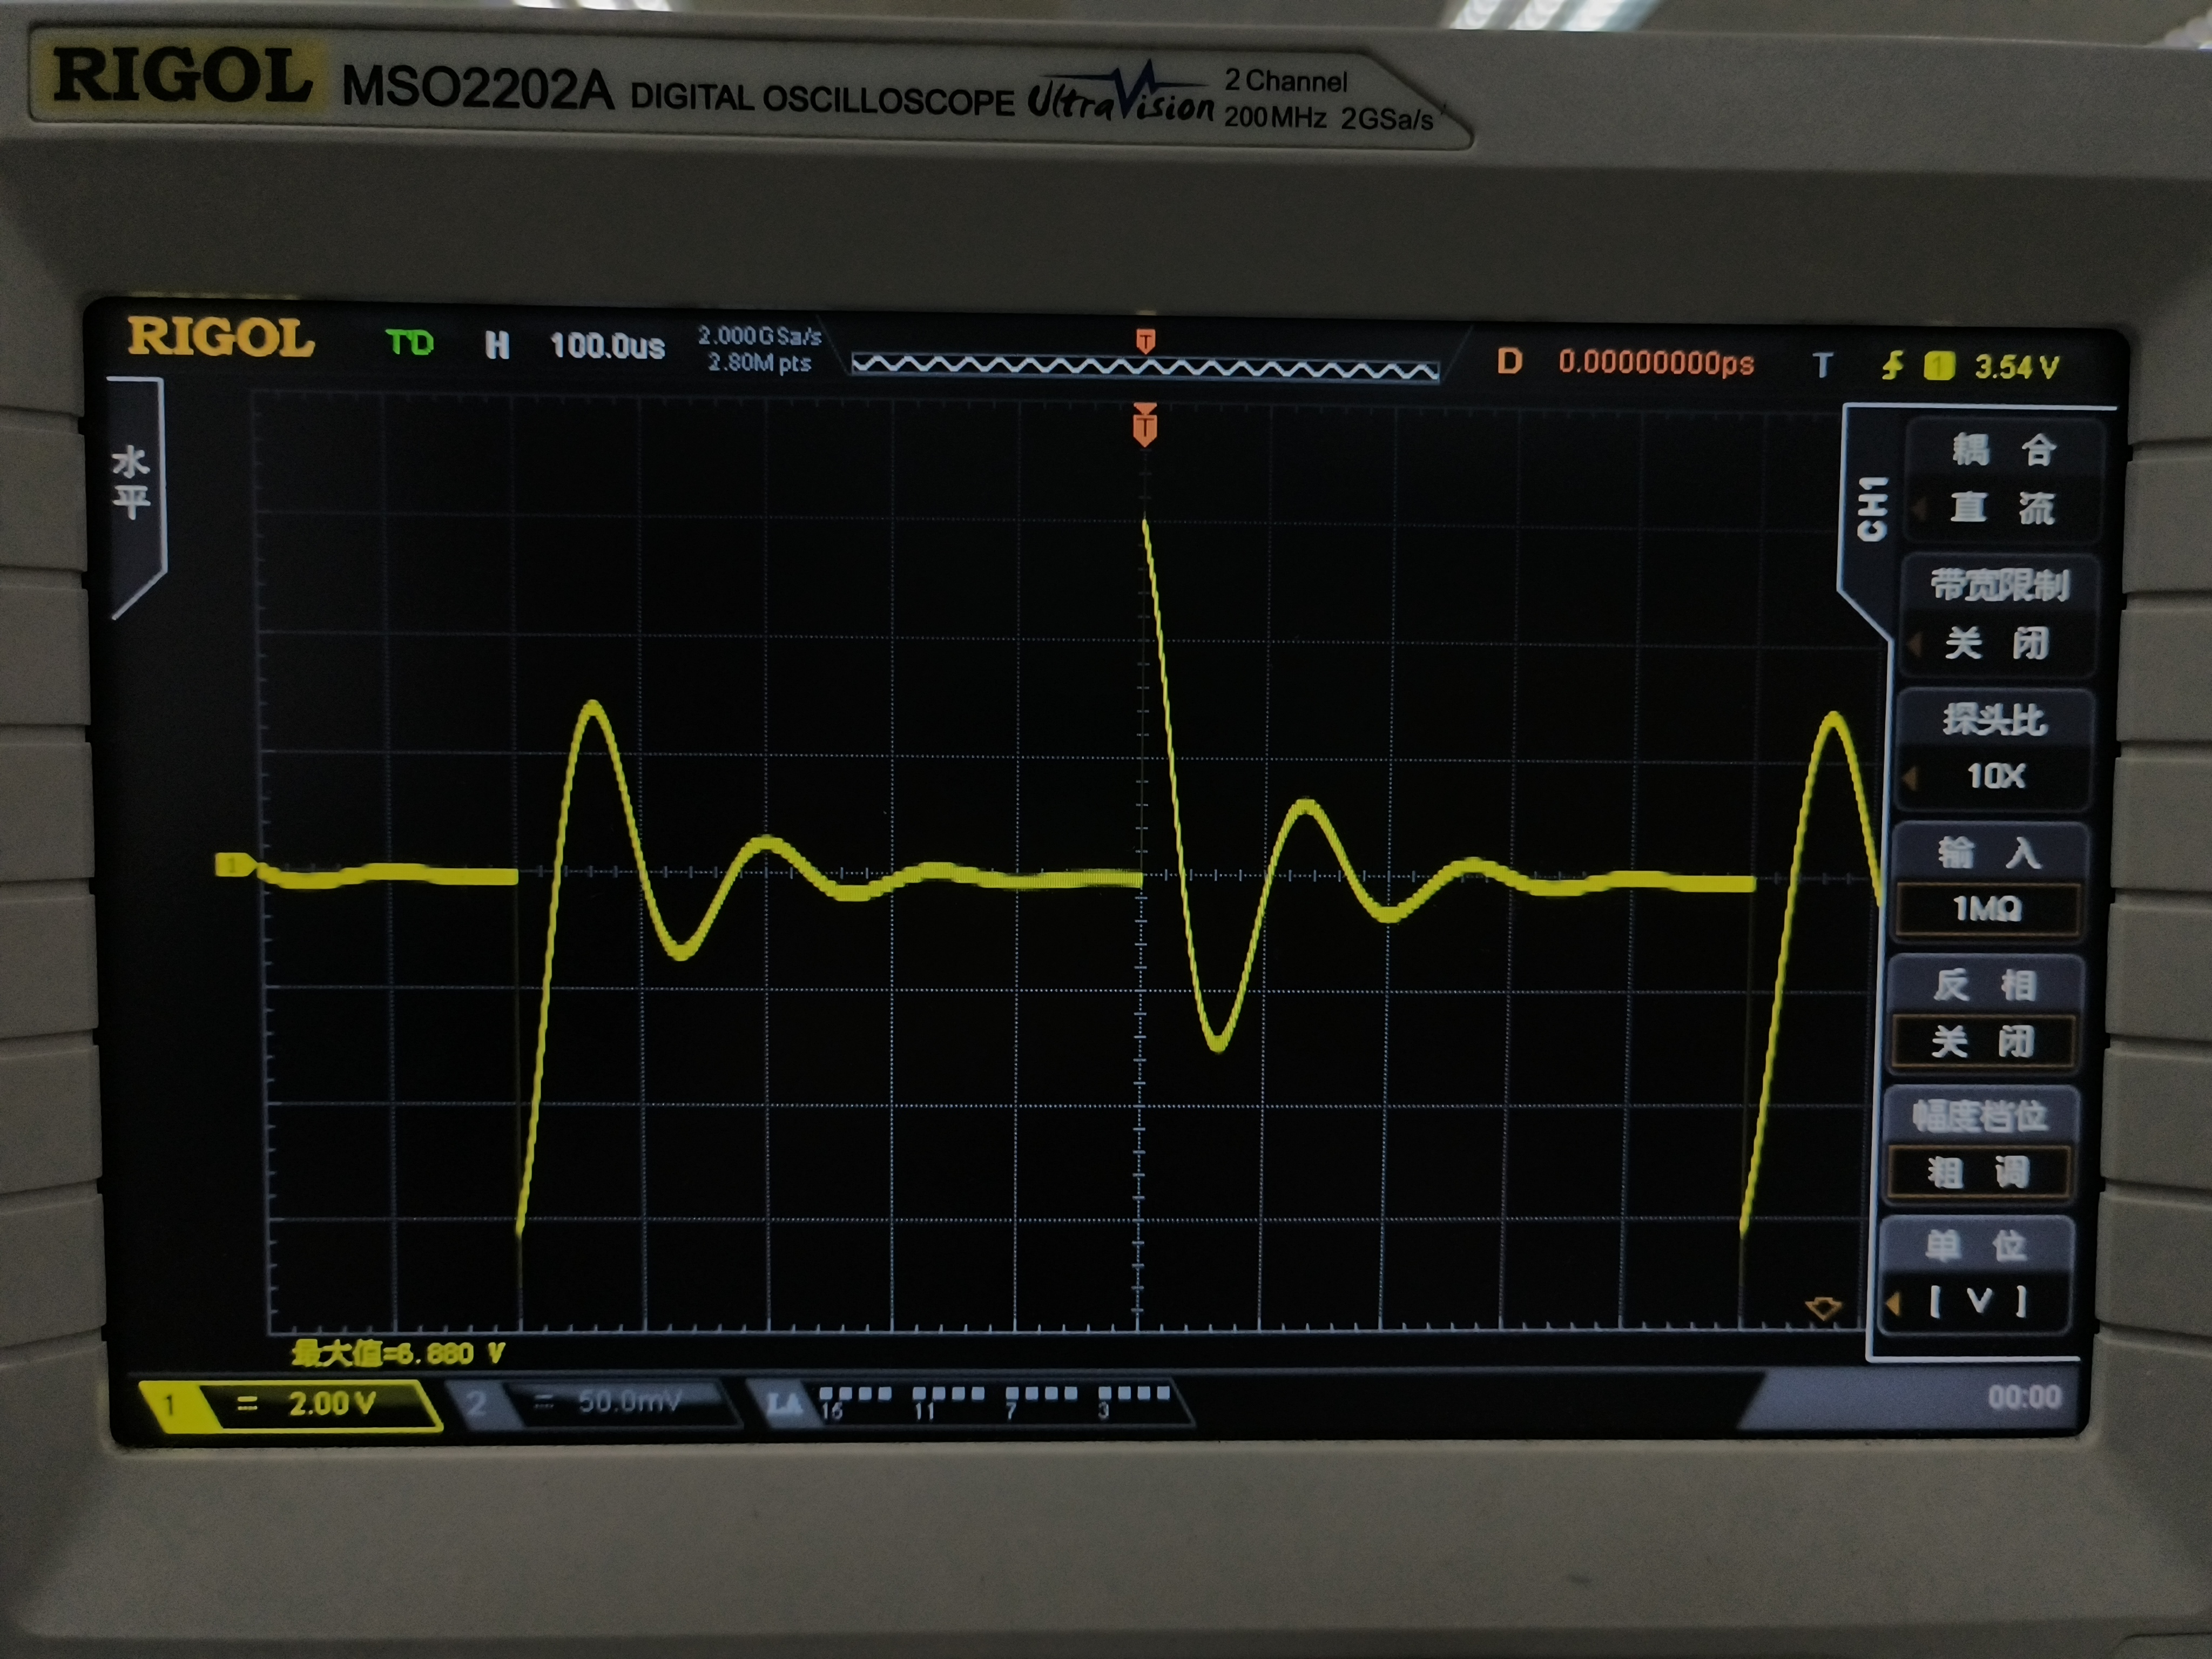
\includegraphics[width=0.43\textwidth]{2b.jpg}}\\
            \subfloat[$U_L$]{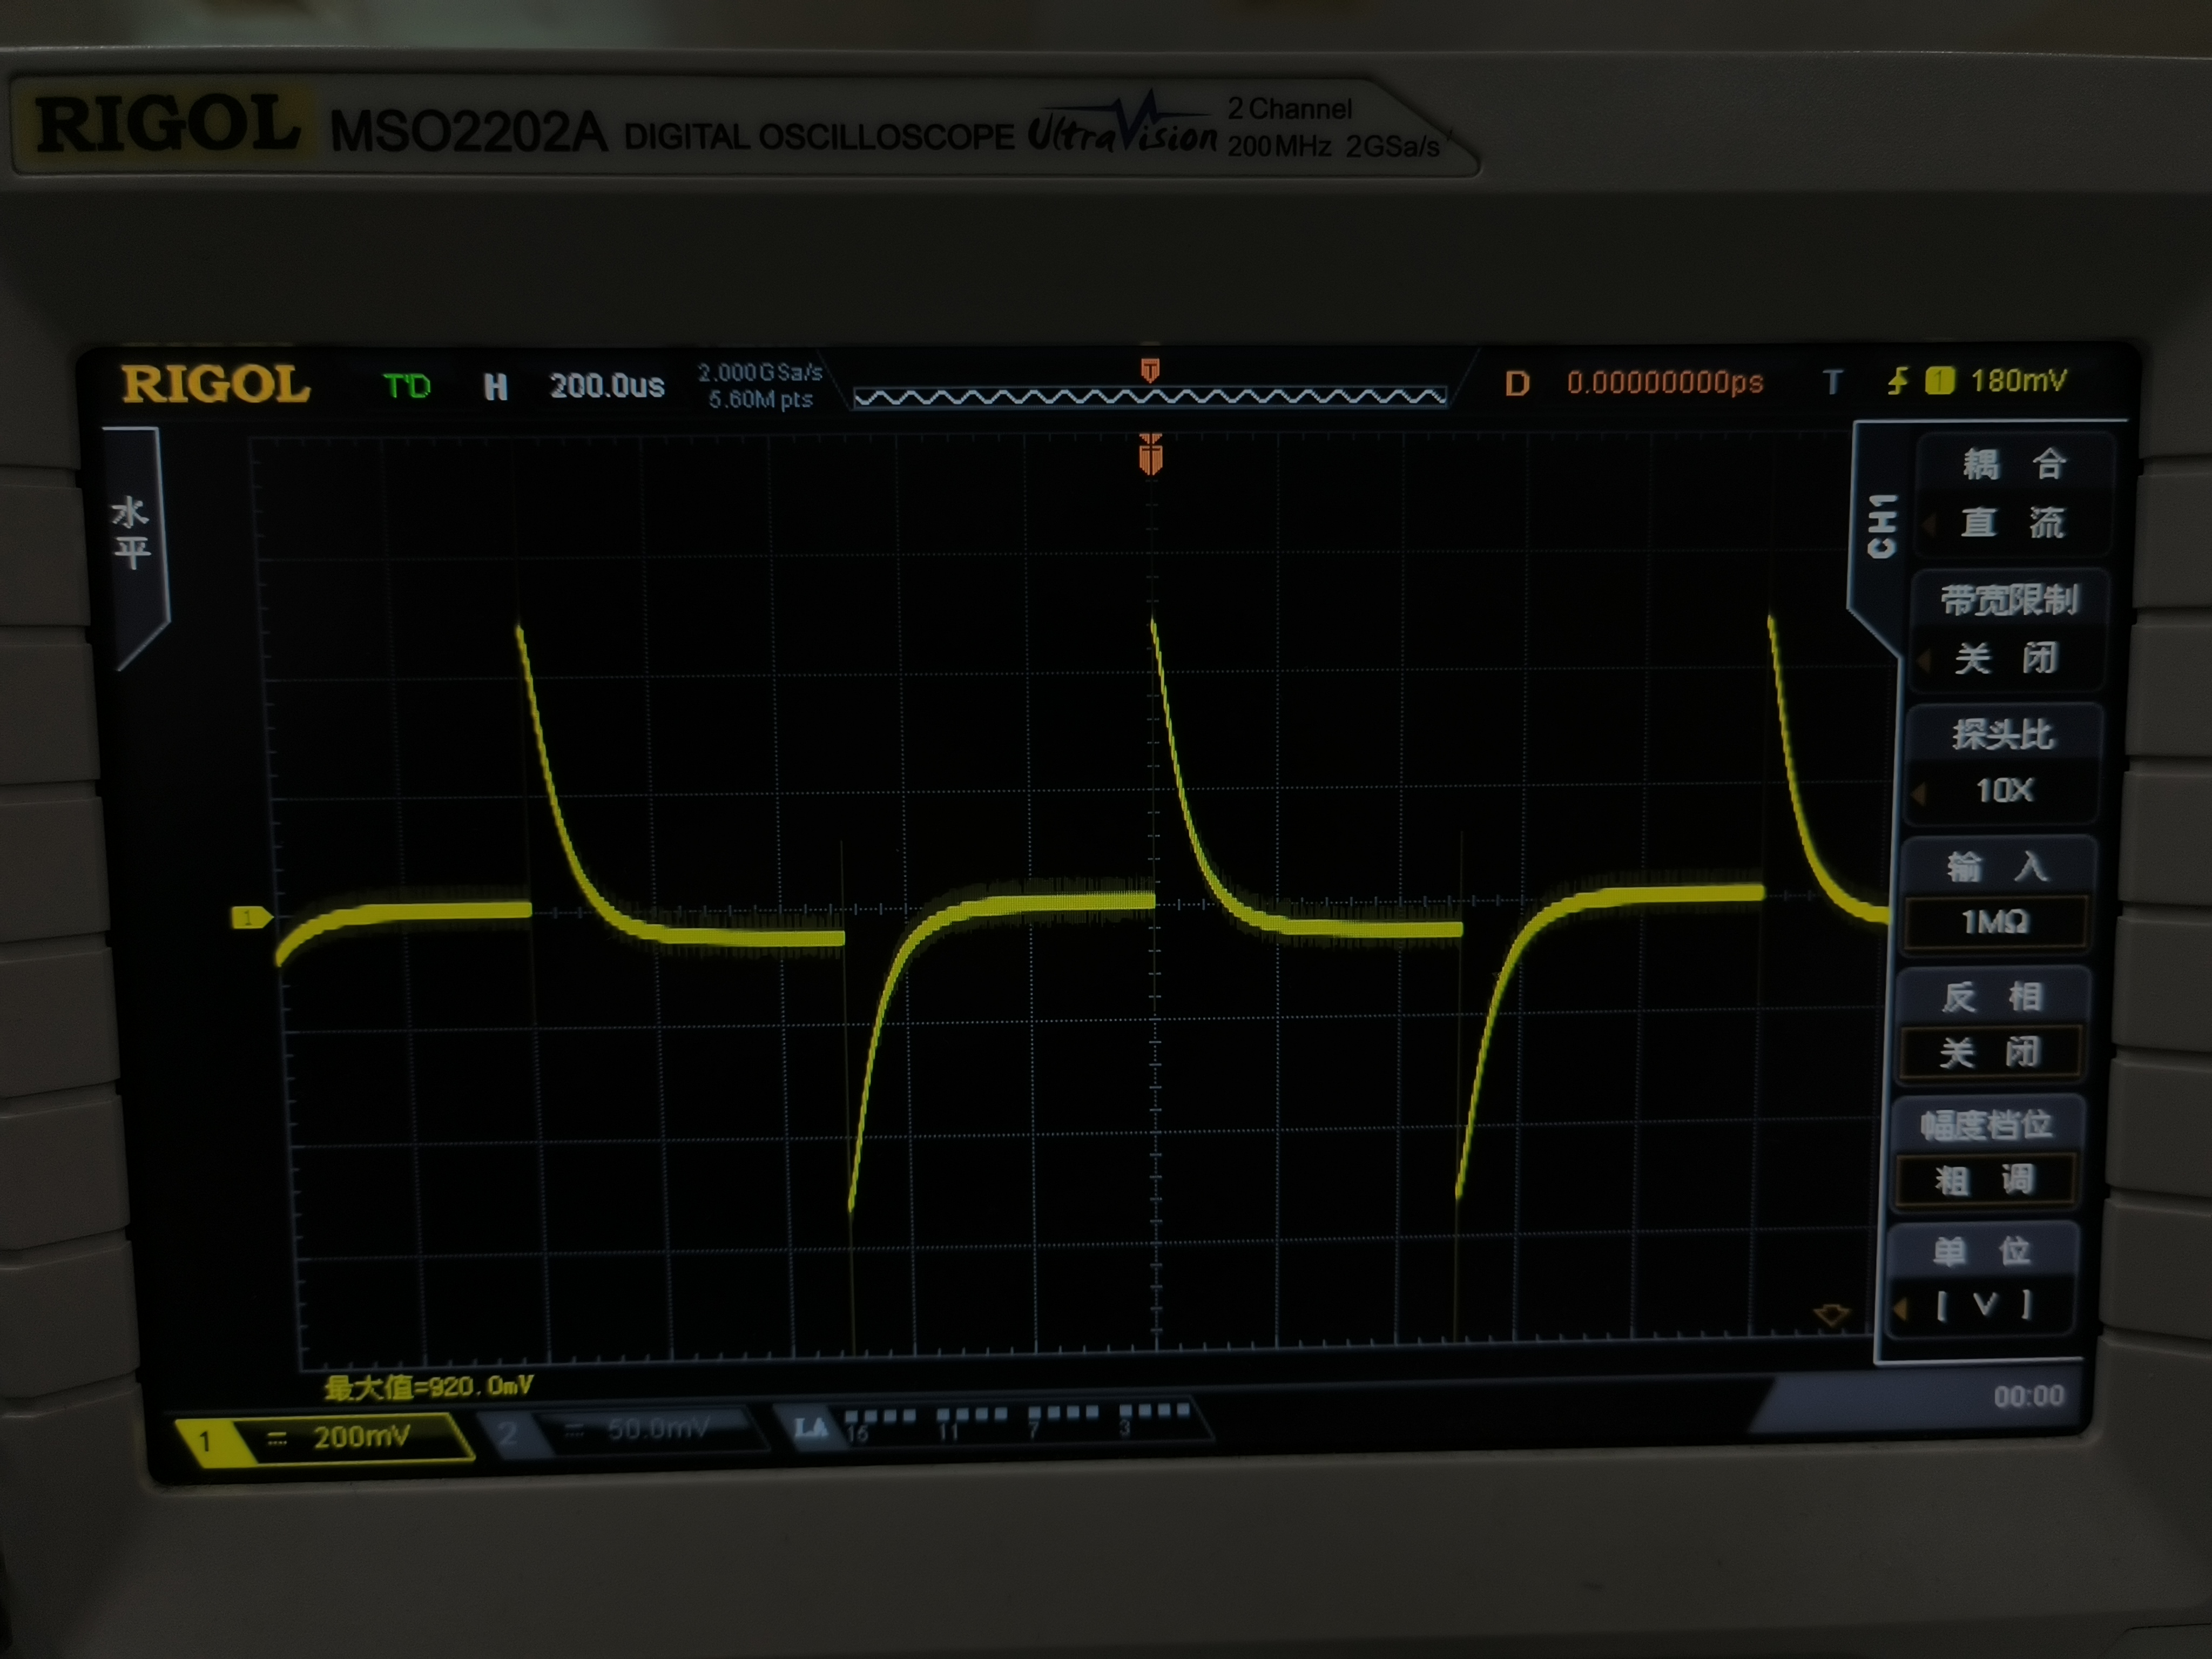
\includegraphics[width=0.43\textwidth]{2c.jpg}}\hspace{6mm}
            \subfloat[$U_R$]{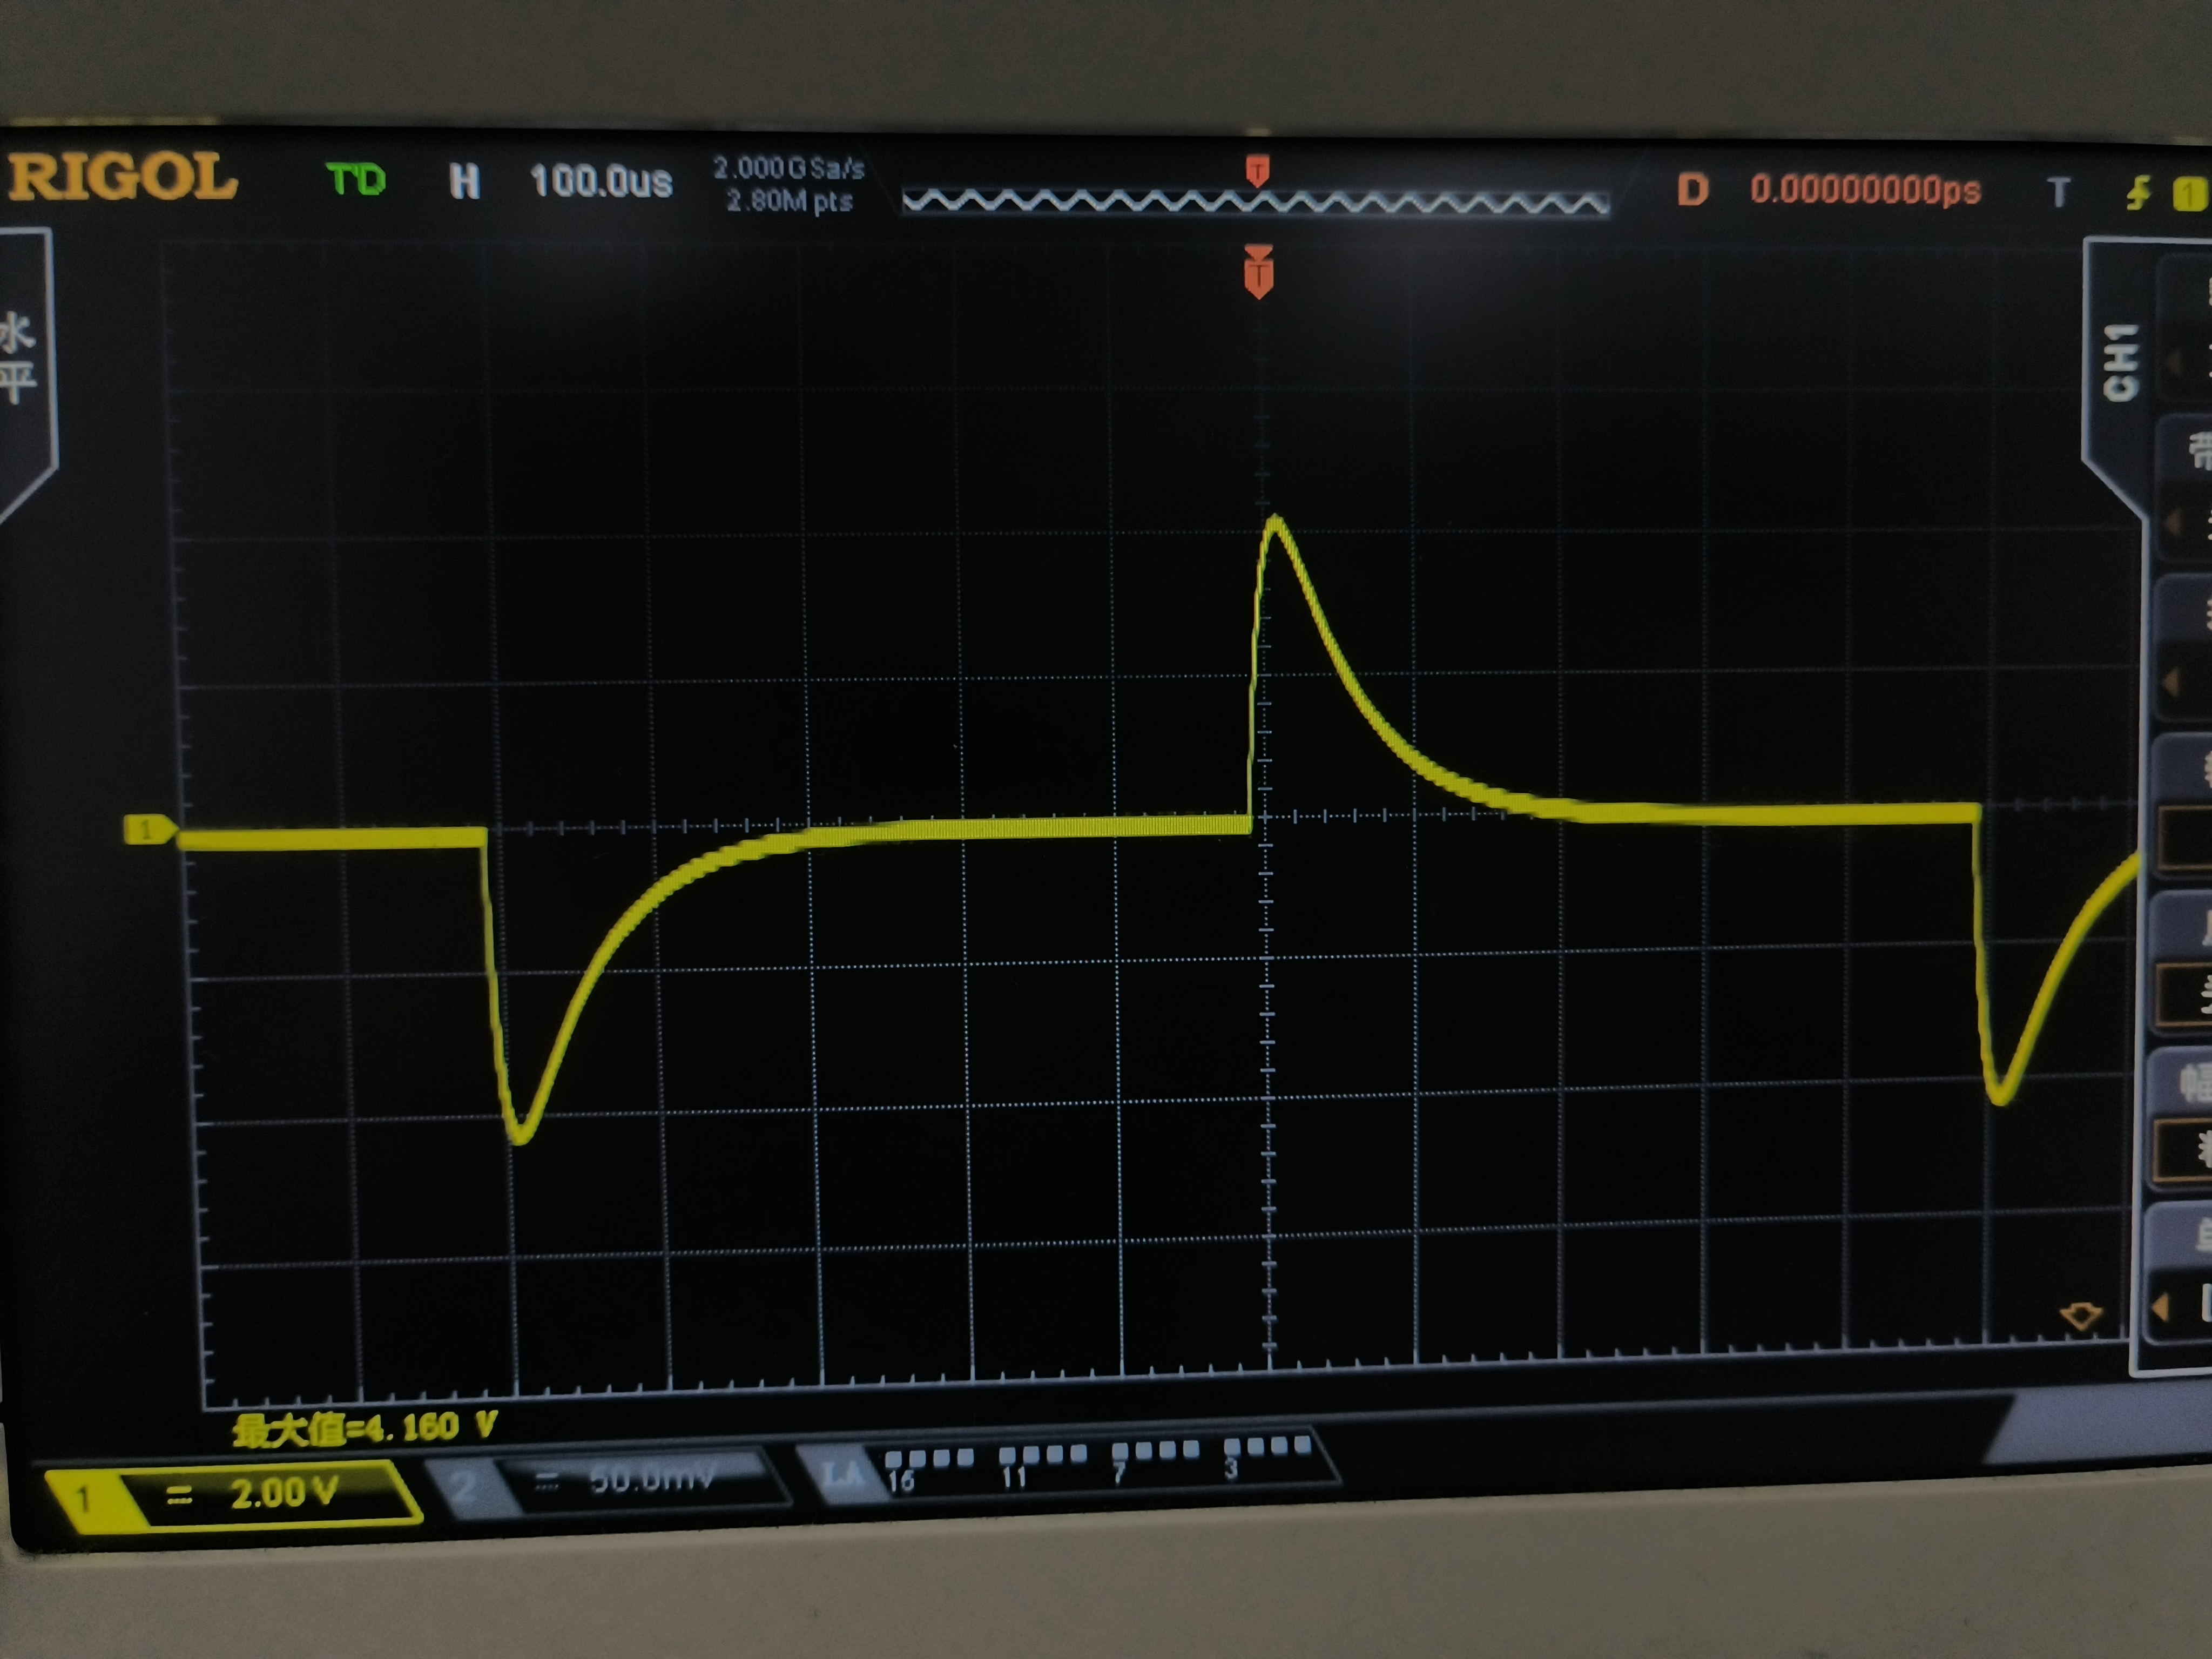
\includegraphics[width=0.43\textwidth]{2d.jpg}}
            \caption{$R=510\unit{\ohm}$(过阻尼)}
        \end{figure}\par
        ~
        \begin{figure}[!ht]
            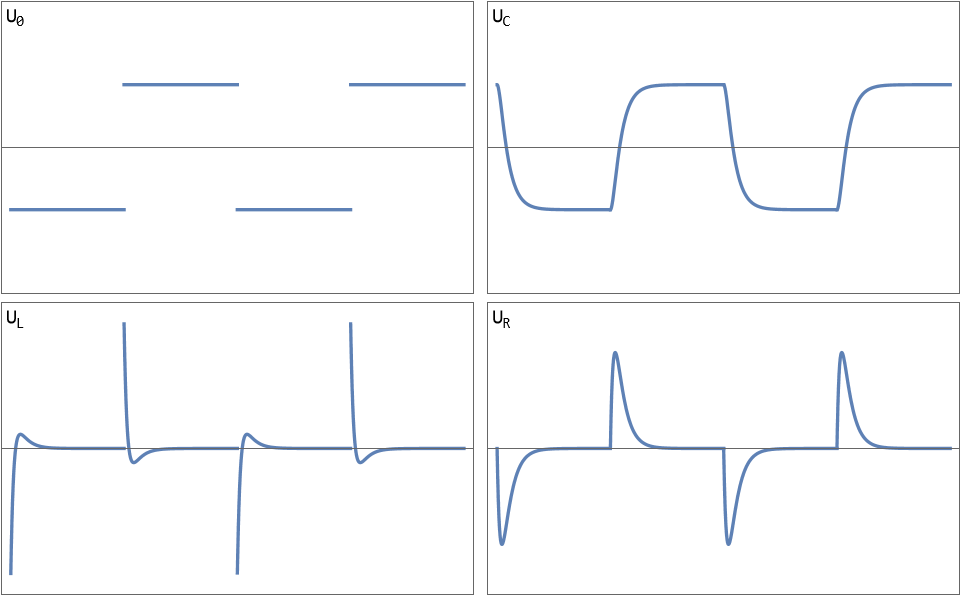
\includegraphics[width=0.9\textwidth]{2e.png}
            \caption{理论计算结果}
        \end{figure}\par

        \begin{figure}[!ht]
            \subfloat[$U_0$]{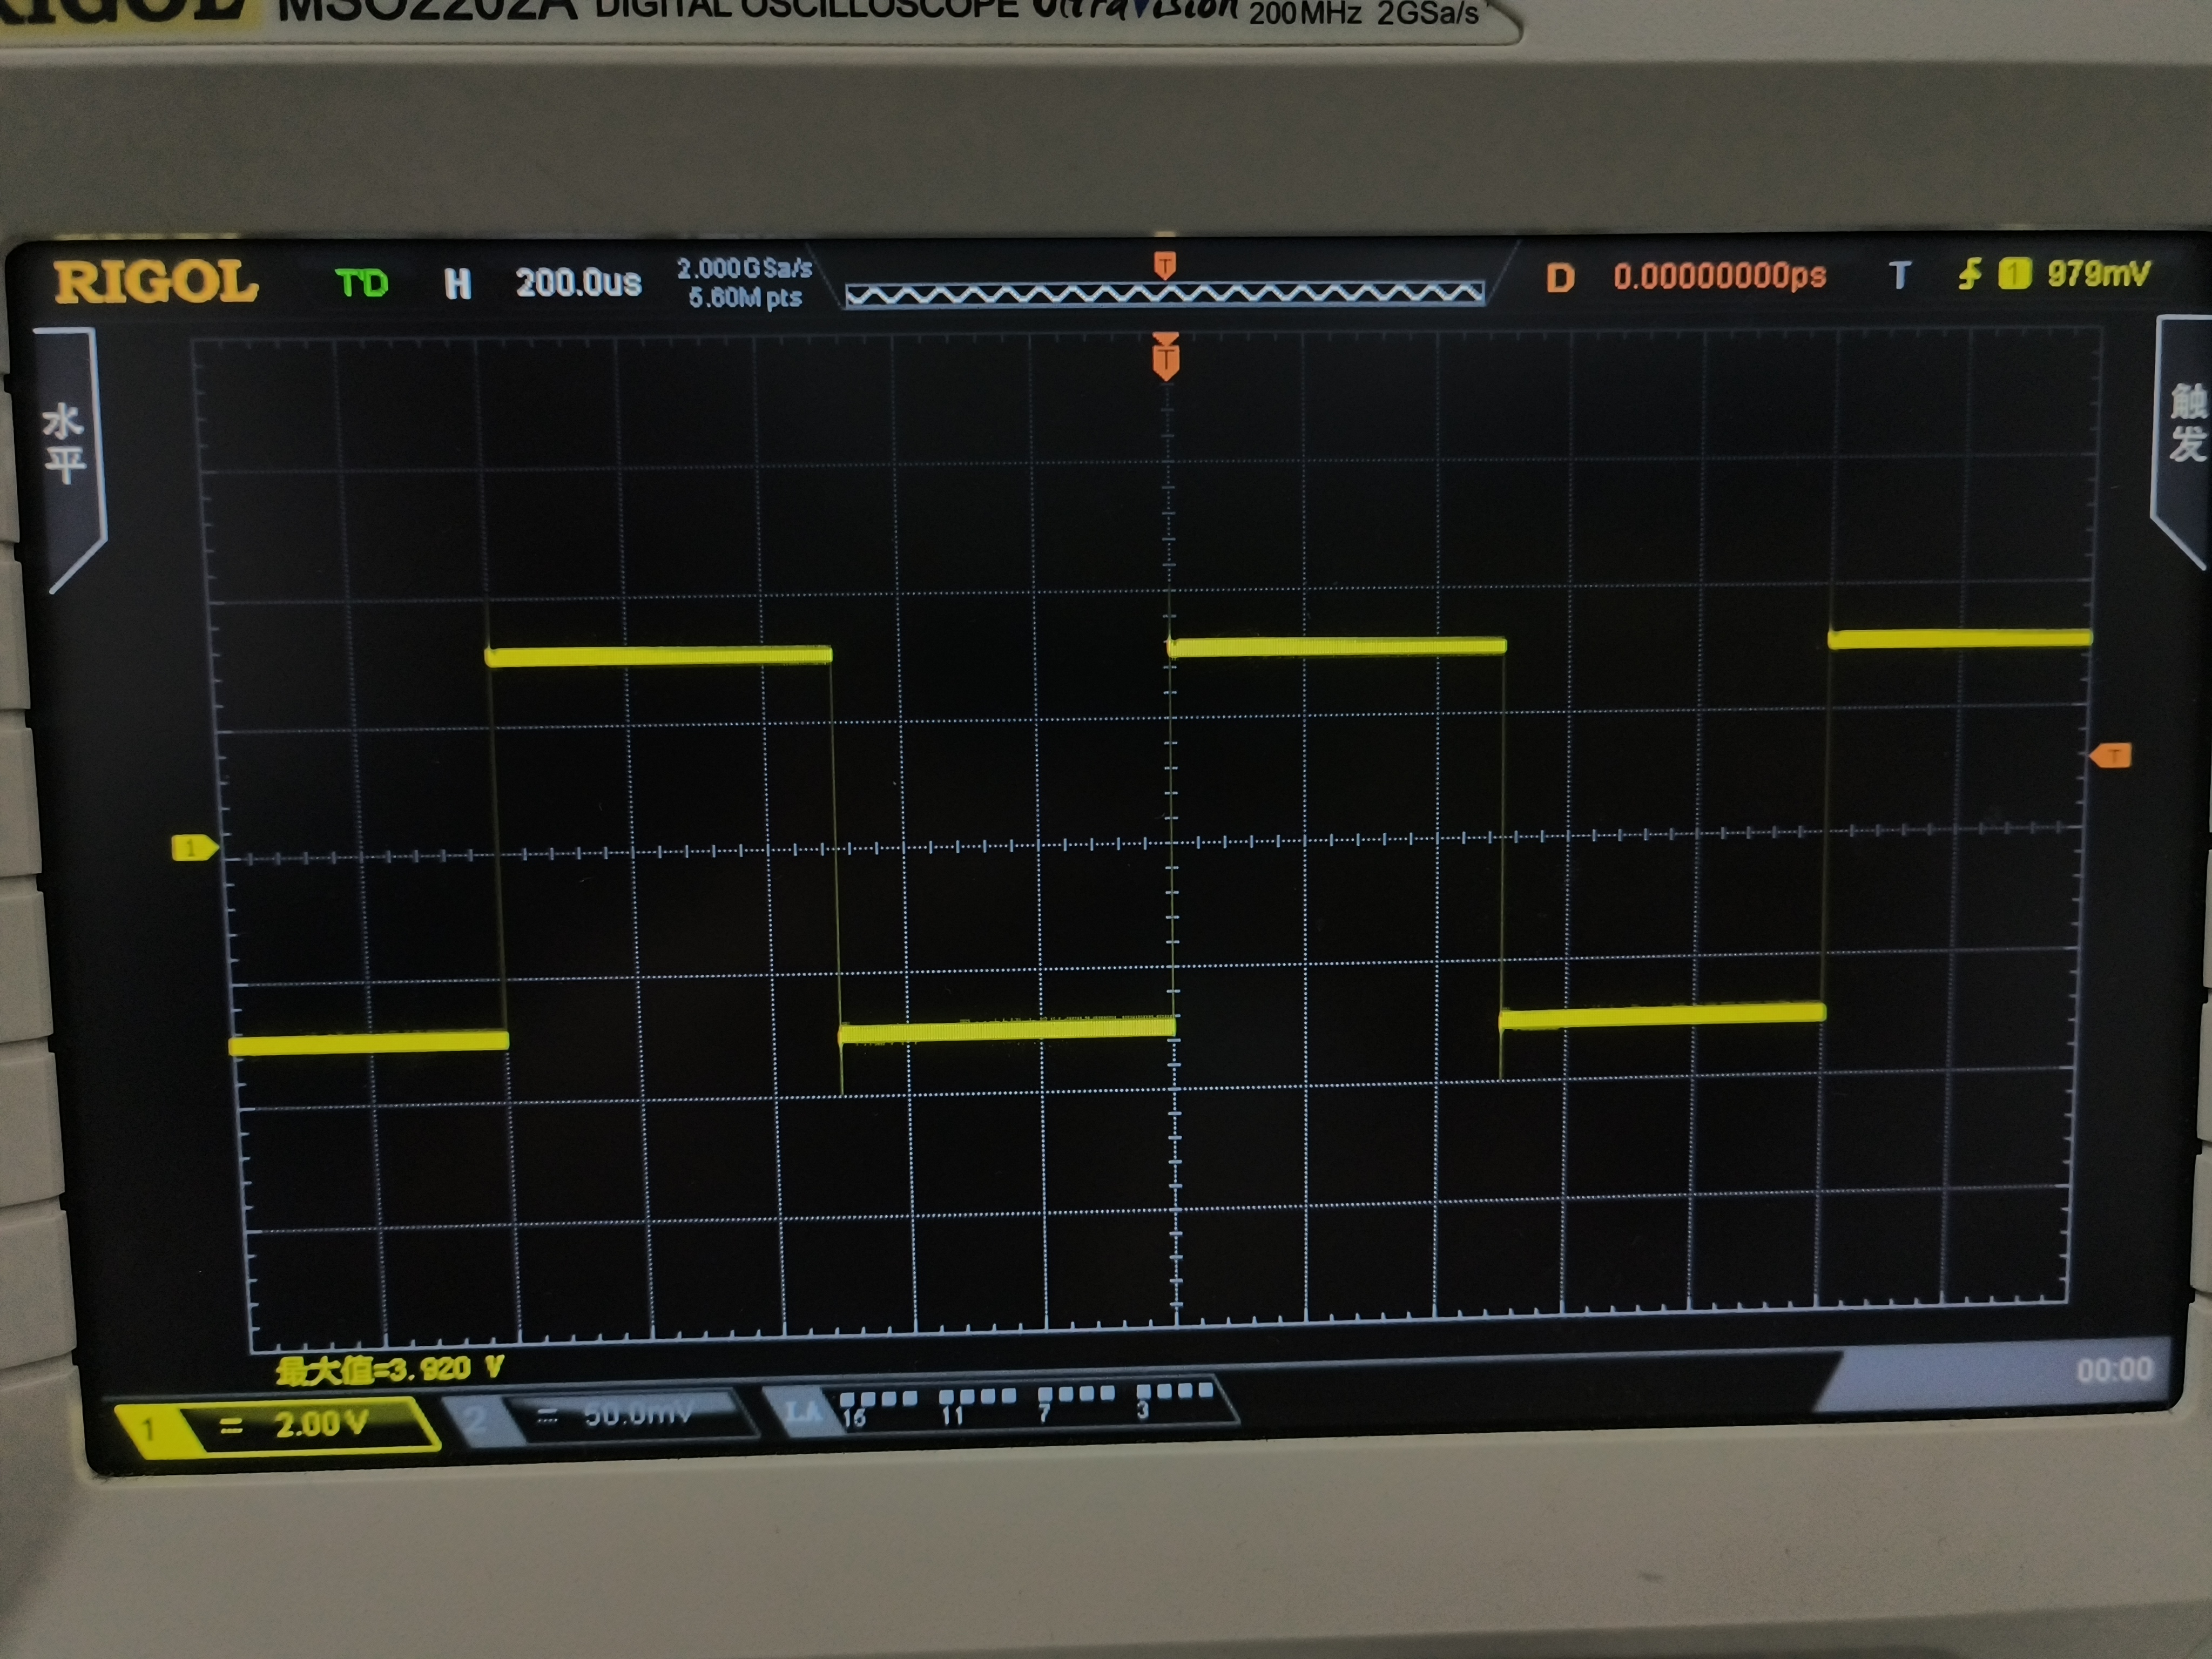
\includegraphics[width=0.43\textwidth]{sq.jpg}}\hspace{6mm}
            \subfloat[$U_C$]{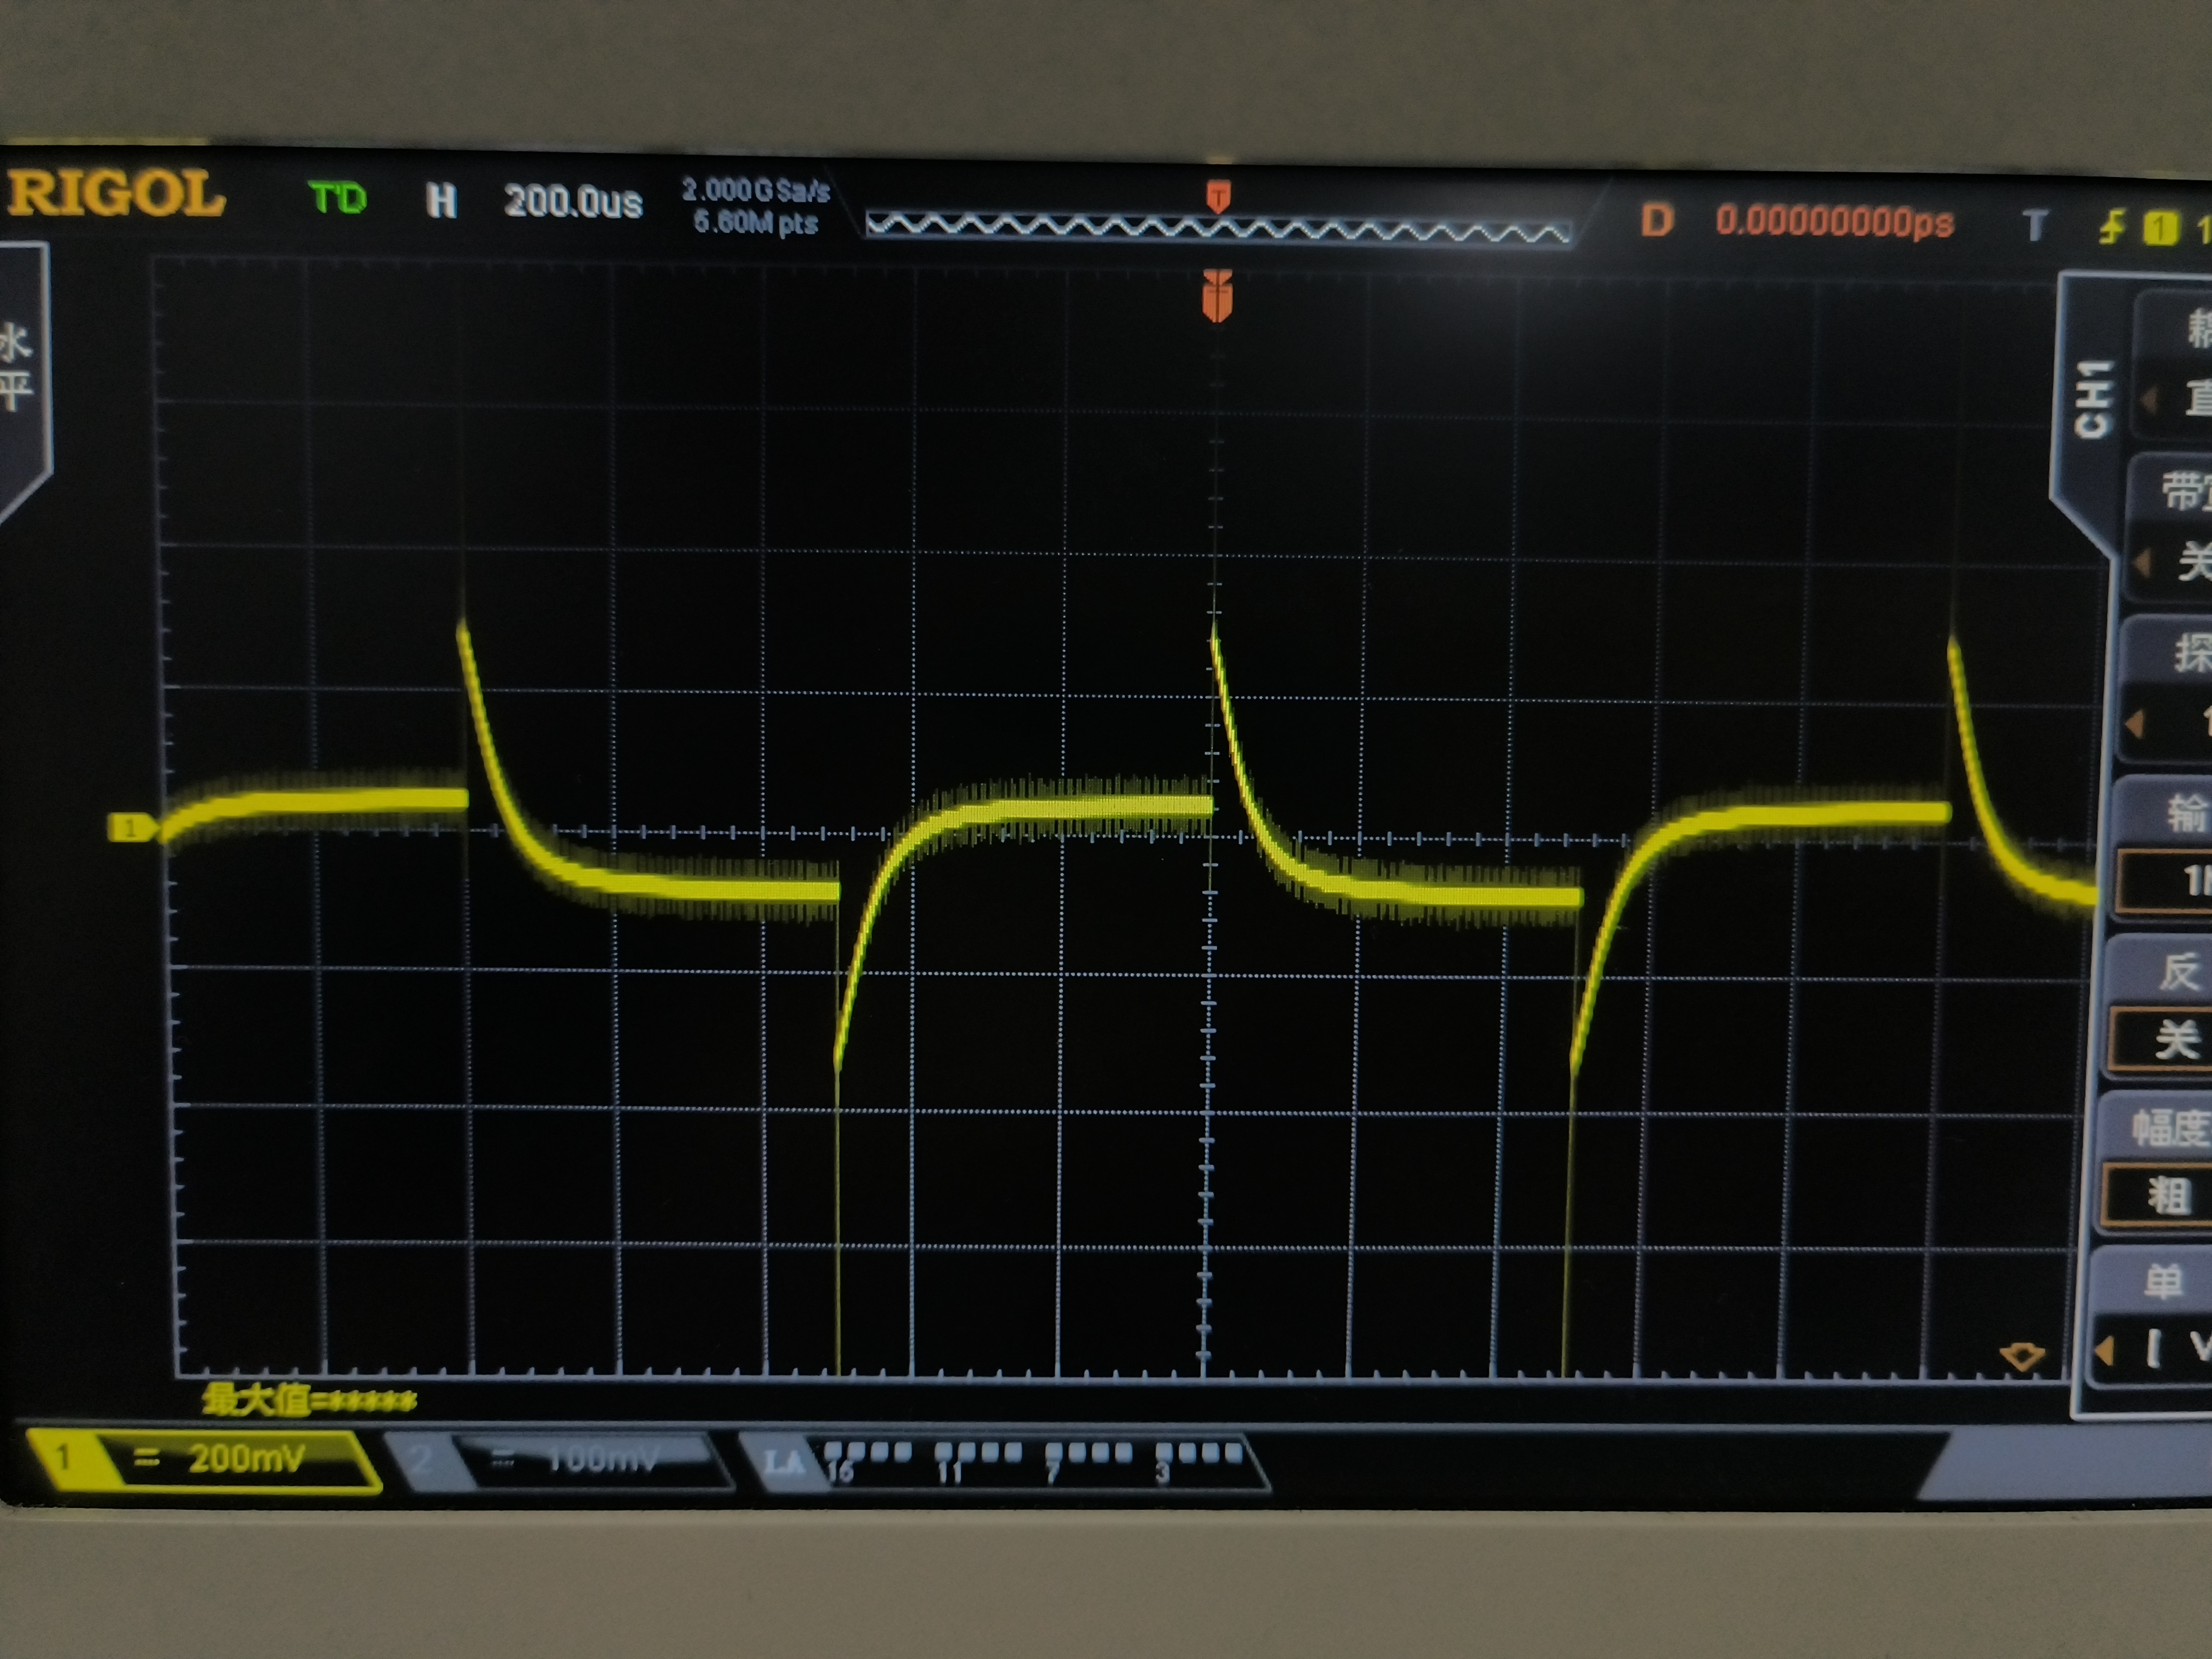
\includegraphics[width=0.43\textwidth]{3b.jpg}}\\
            \subfloat[$U_L$]{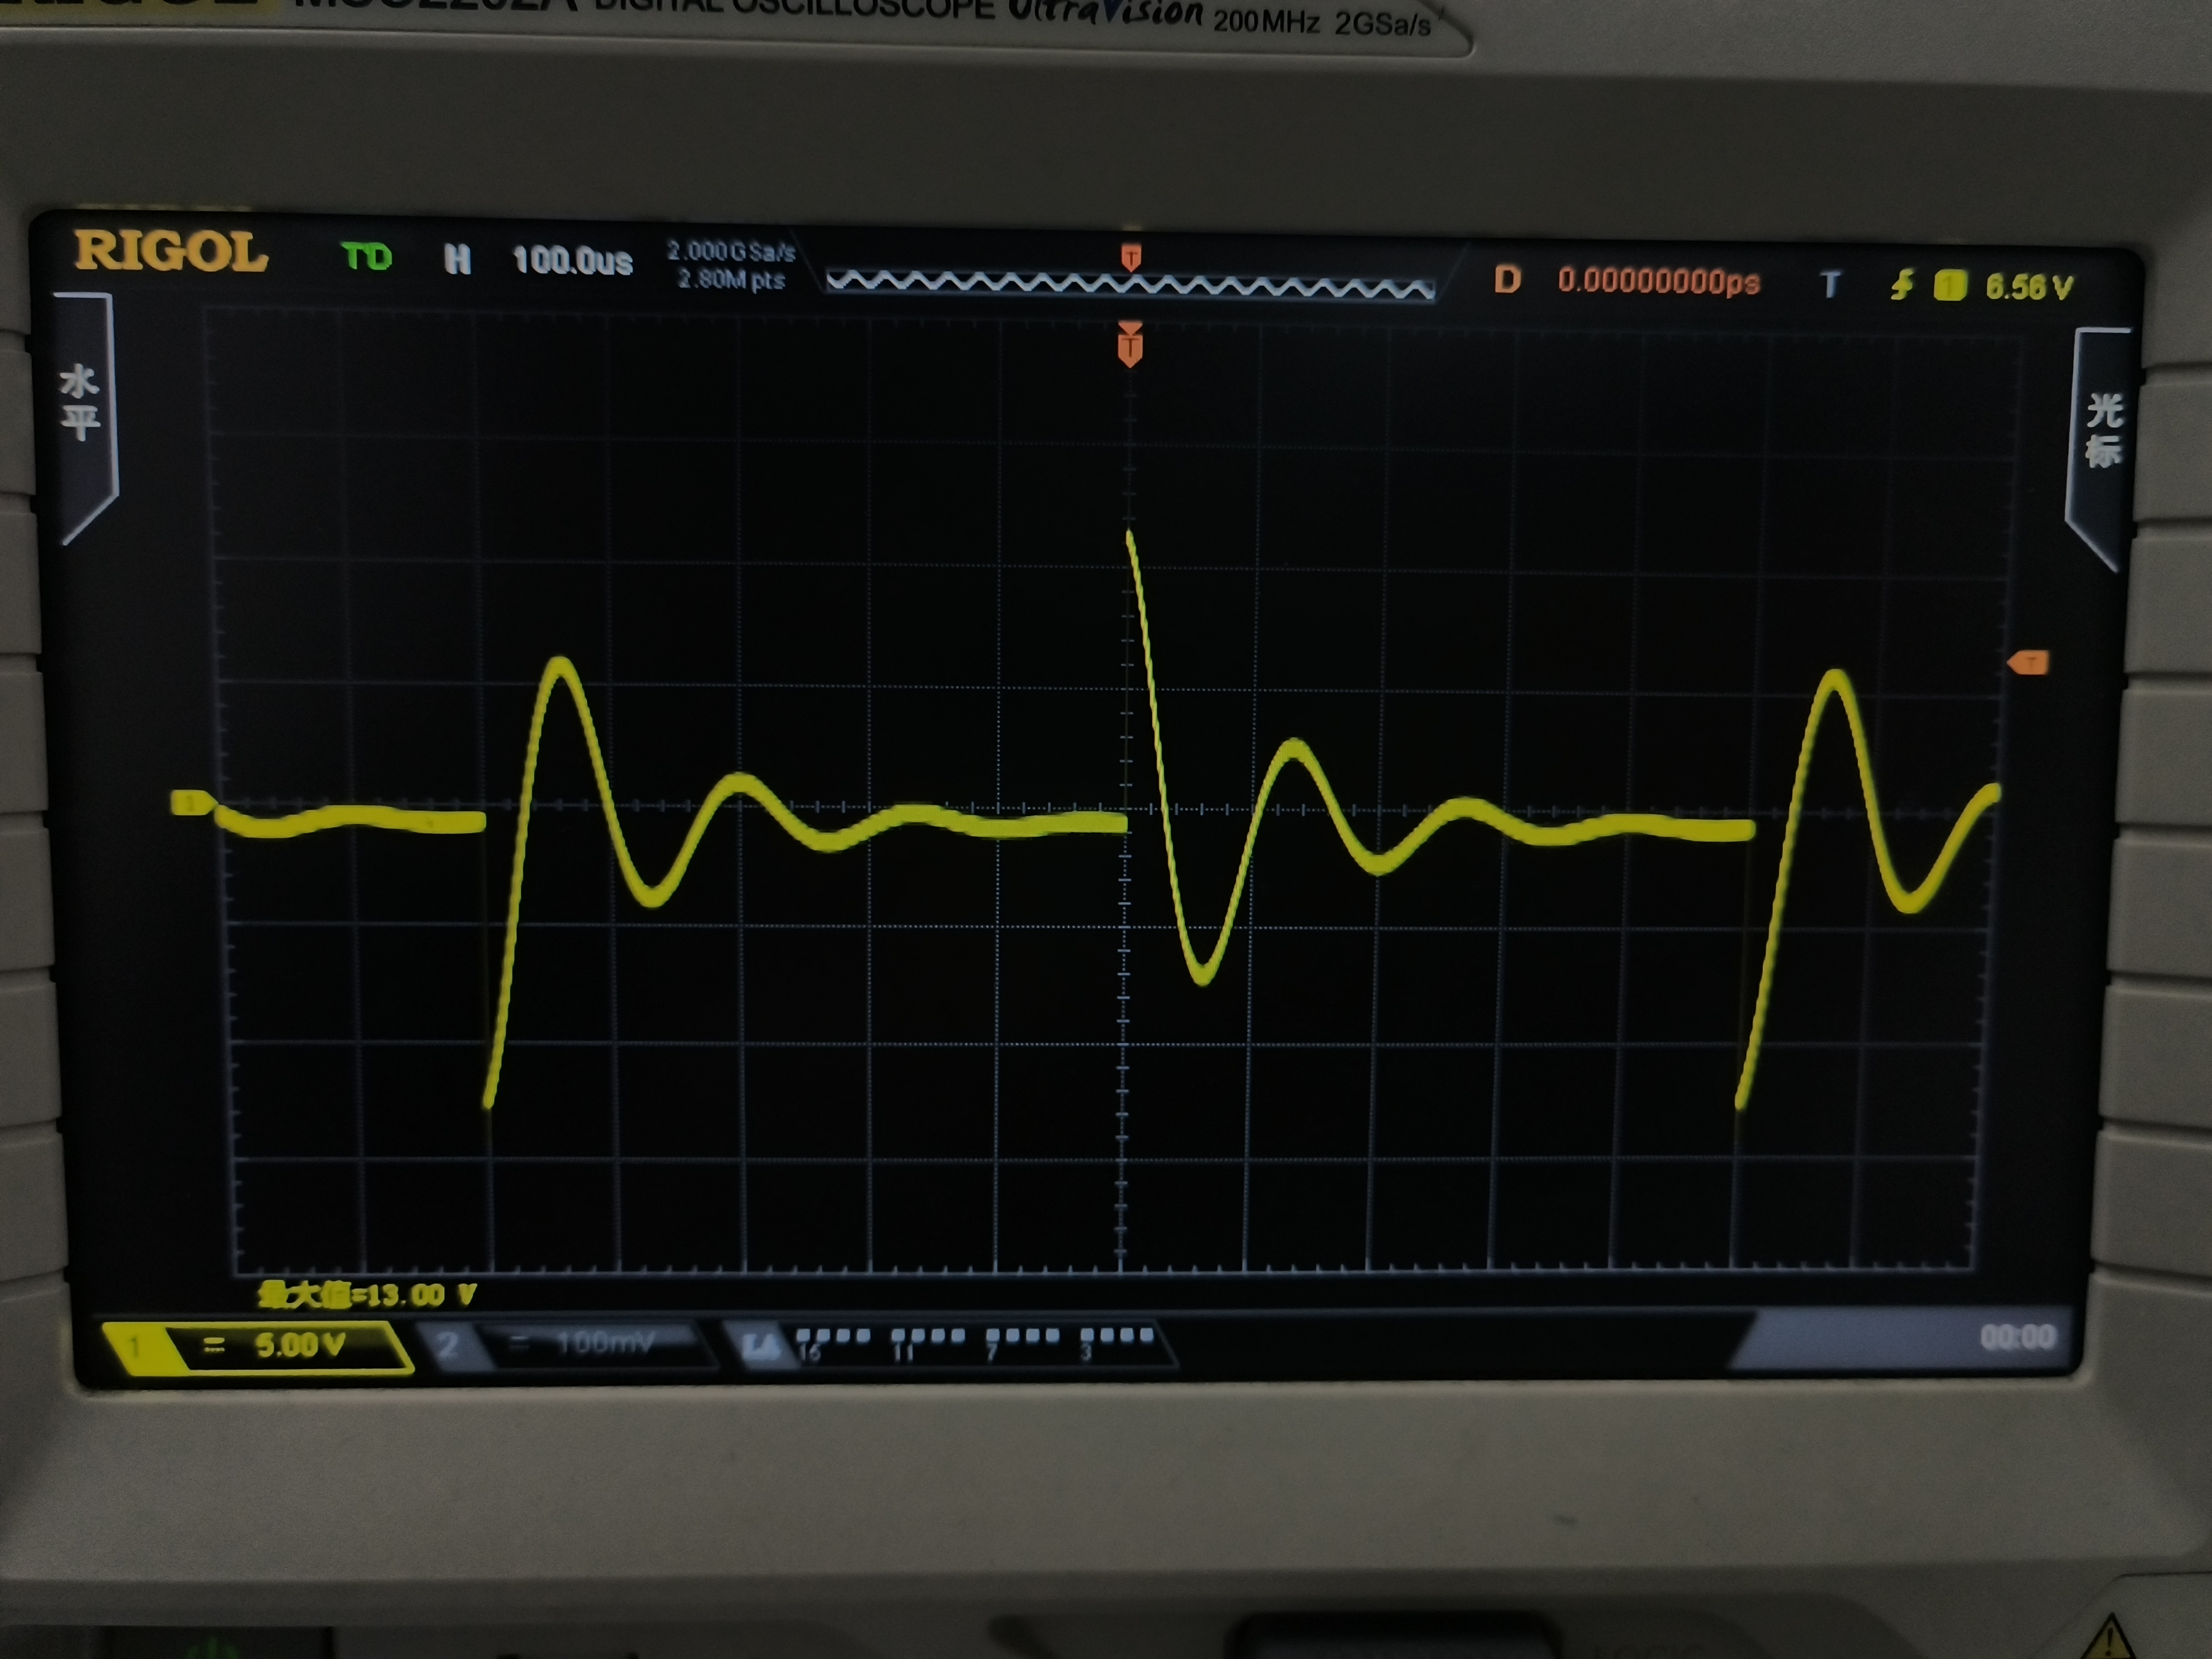
\includegraphics[width=0.43\textwidth]{3c.jpg}}\hspace{6mm}
            \subfloat[$U_R$]{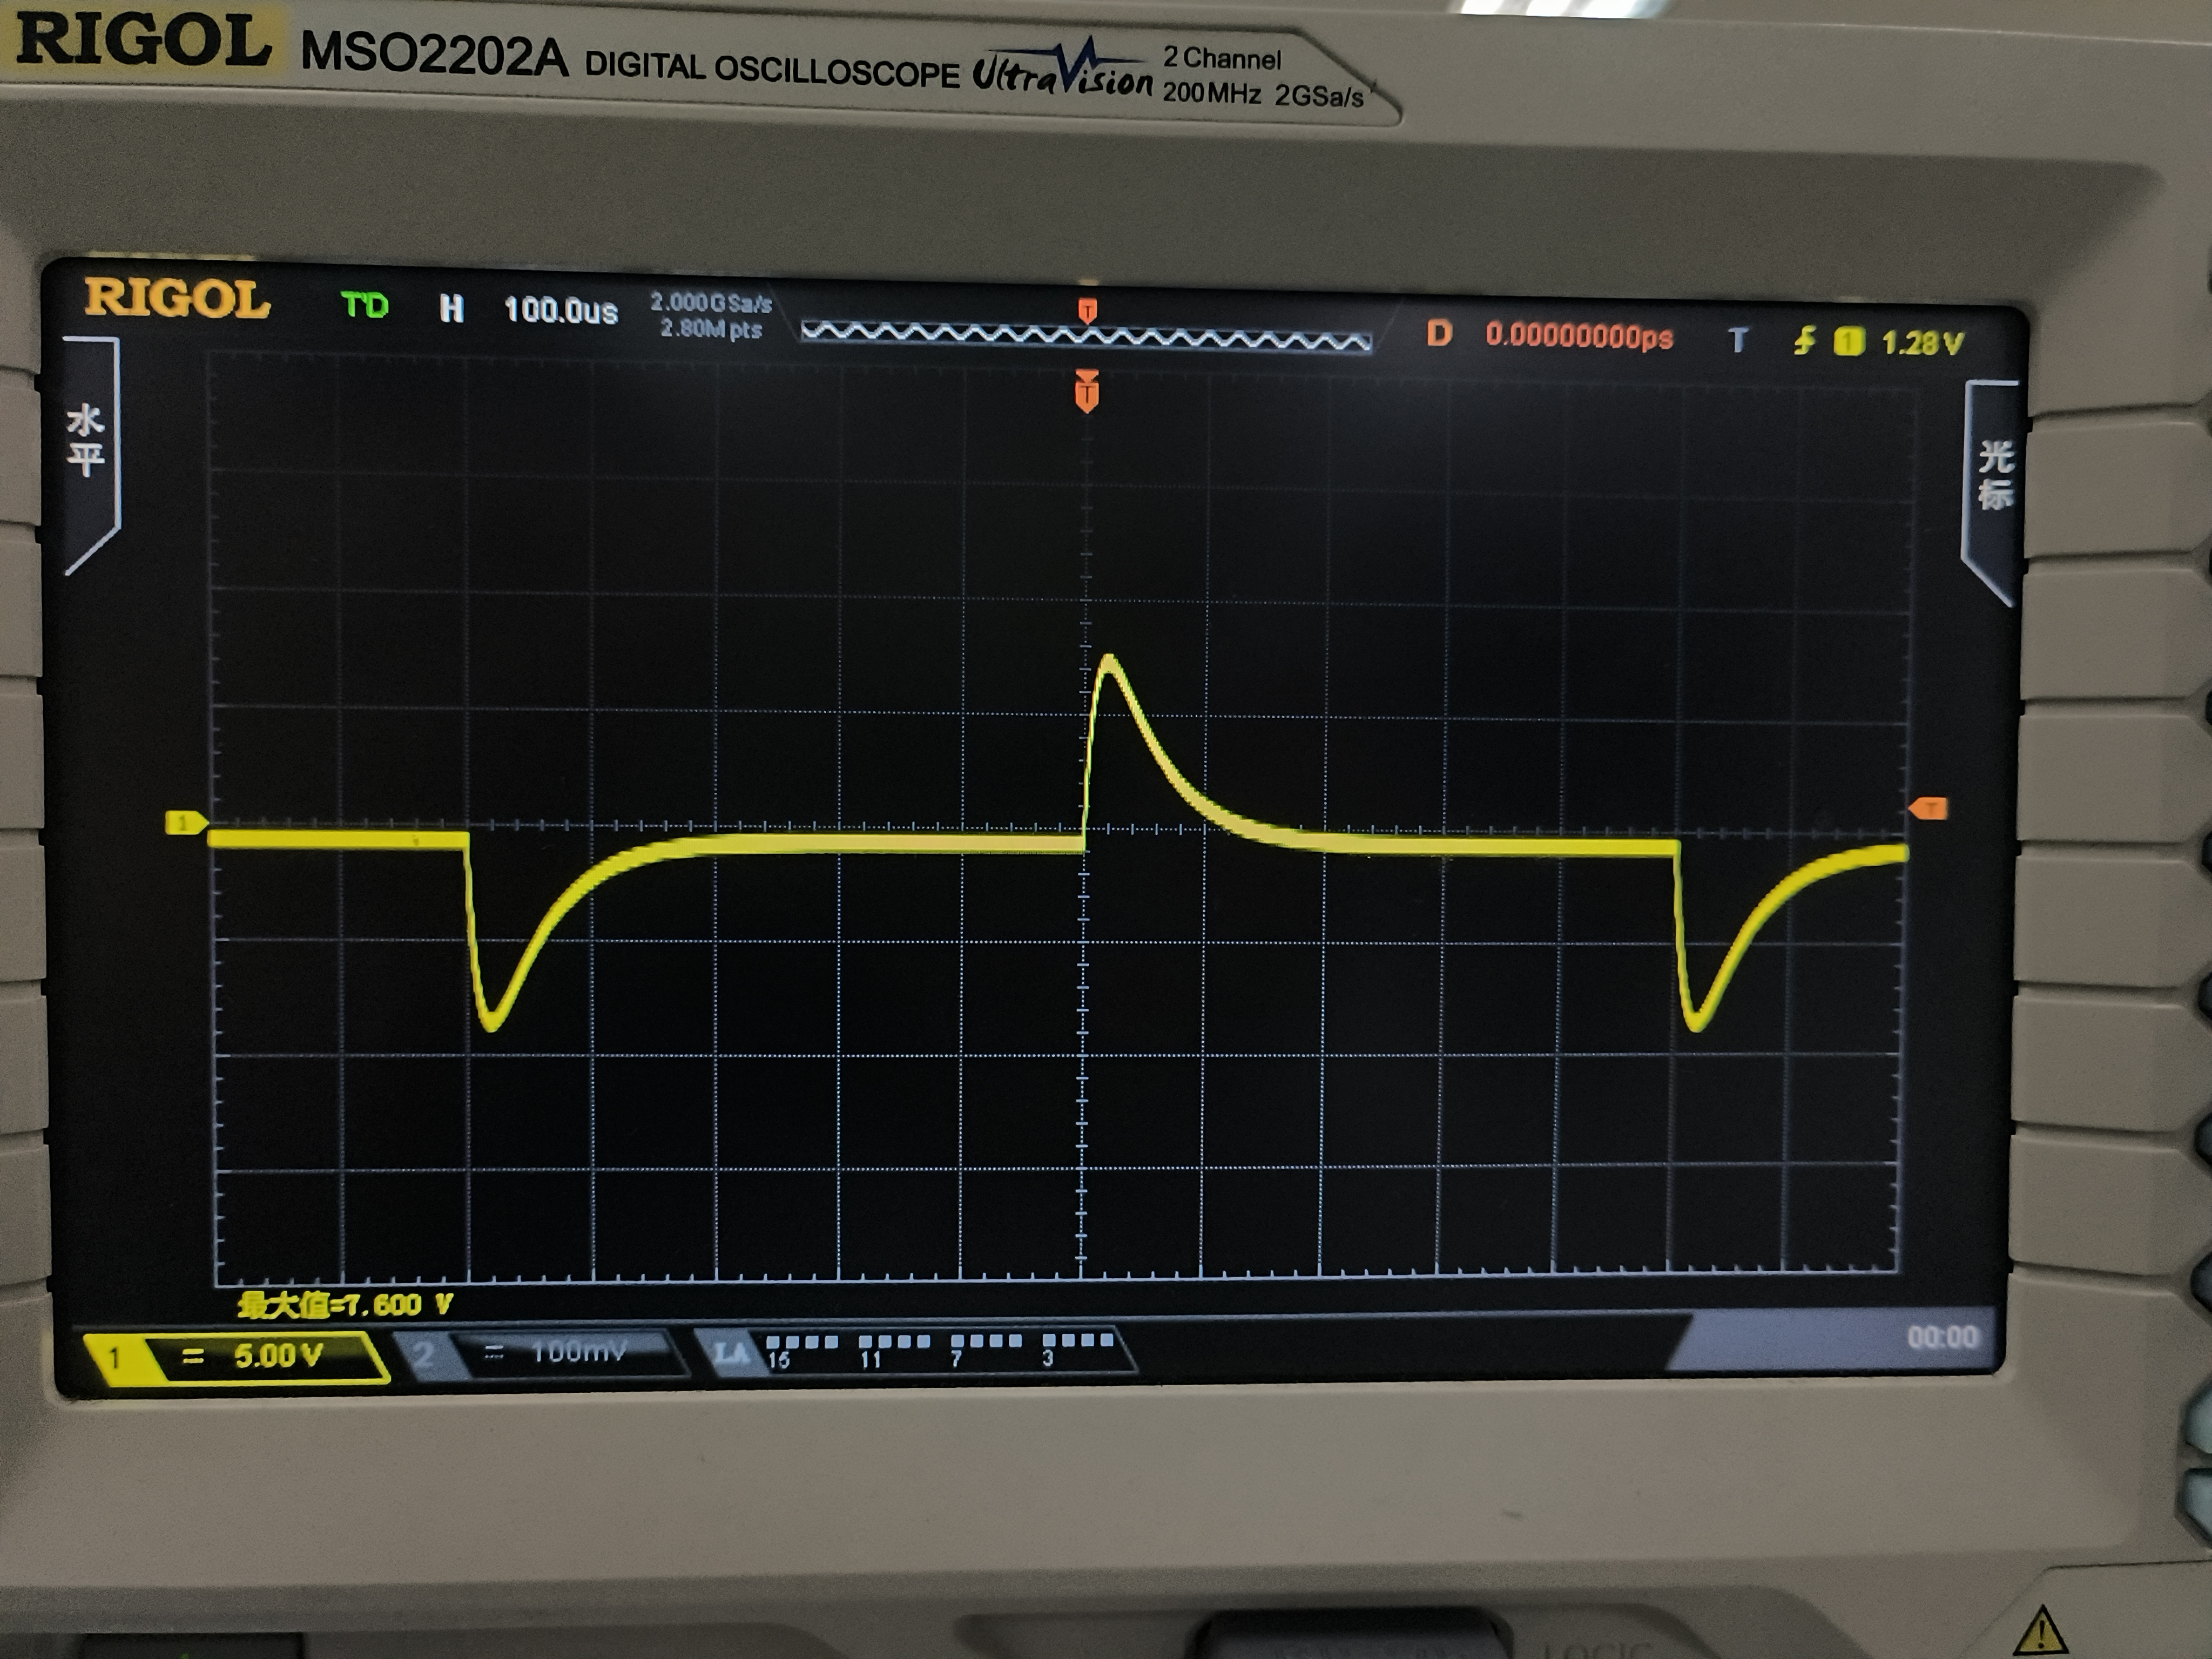
\includegraphics[width=0.43\textwidth]{3d.jpg}}
            \caption{$R=447\unit{\ohm}$(临界阻尼)}
        \end{figure}\par
        ~
        \begin{figure}[!ht]
            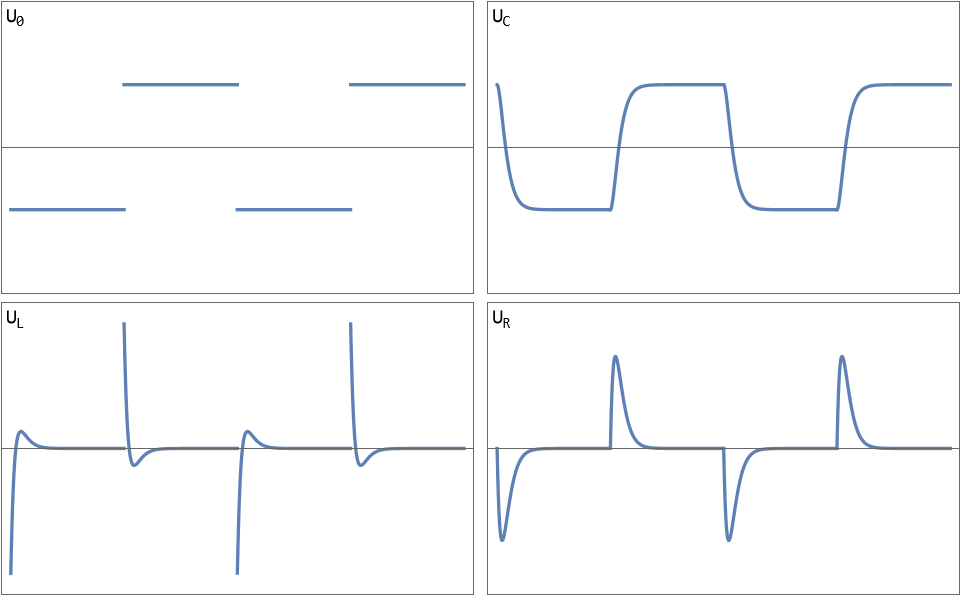
\includegraphics[width=0.9\textwidth]{3e.png}
            \caption{理论计算结果}
        \end{figure}
        \newpage
        \newpage


\section{实验分析}
    \subsection{分析}
    由理论计算图与实际测量结果进行比对,可以发现测量结果与理论有一定偏差,尤其是电容跟电感这两个对频率敏感的元件。在实验中尽管我们多次重新接线,换用不同的导线均没有办法解决这个问题。通过观察函数发生器输出的波形,可以看出输出的方波在切换的时候有很明显的纹波,这很有可能是影响电容电感波形的重要因素。在电源高频开关的时候,输出波形中会附带有一些随机噪声和高频纹波,一般是MHz级别的,这时候如果使用带通滤波器或许可以有效的提升结果的准确性。
    \subsection{误差分析}
        \begin{enumerate}
            \item 仪器输出与测量可能产生误差
            \item 线路上的电阻电感电容对结果有一定影响
            \item 示波器的探头可能形成天线接收空间电磁辐射
        \end{enumerate}
\section{思考题}
    方波源频率固定,输出波形相较手动合断更加稳定,便于观测;且如果只有直流源的合断,中间不改变方向,二阶电路将无法回到初始状态,就不会出现周期性的变化。
\section{实验心得}
    本次实验实际观察到了二阶电路的动态过程,但并不完全成功,有很多缺憾之处。这也使我对于动态电路又有了更加清晰明确的认知,同时对于阻抗匹配,电源品质也有更深入的体会。
    \clearpage
    \section{原始数据及图形}
    \begin{center}
        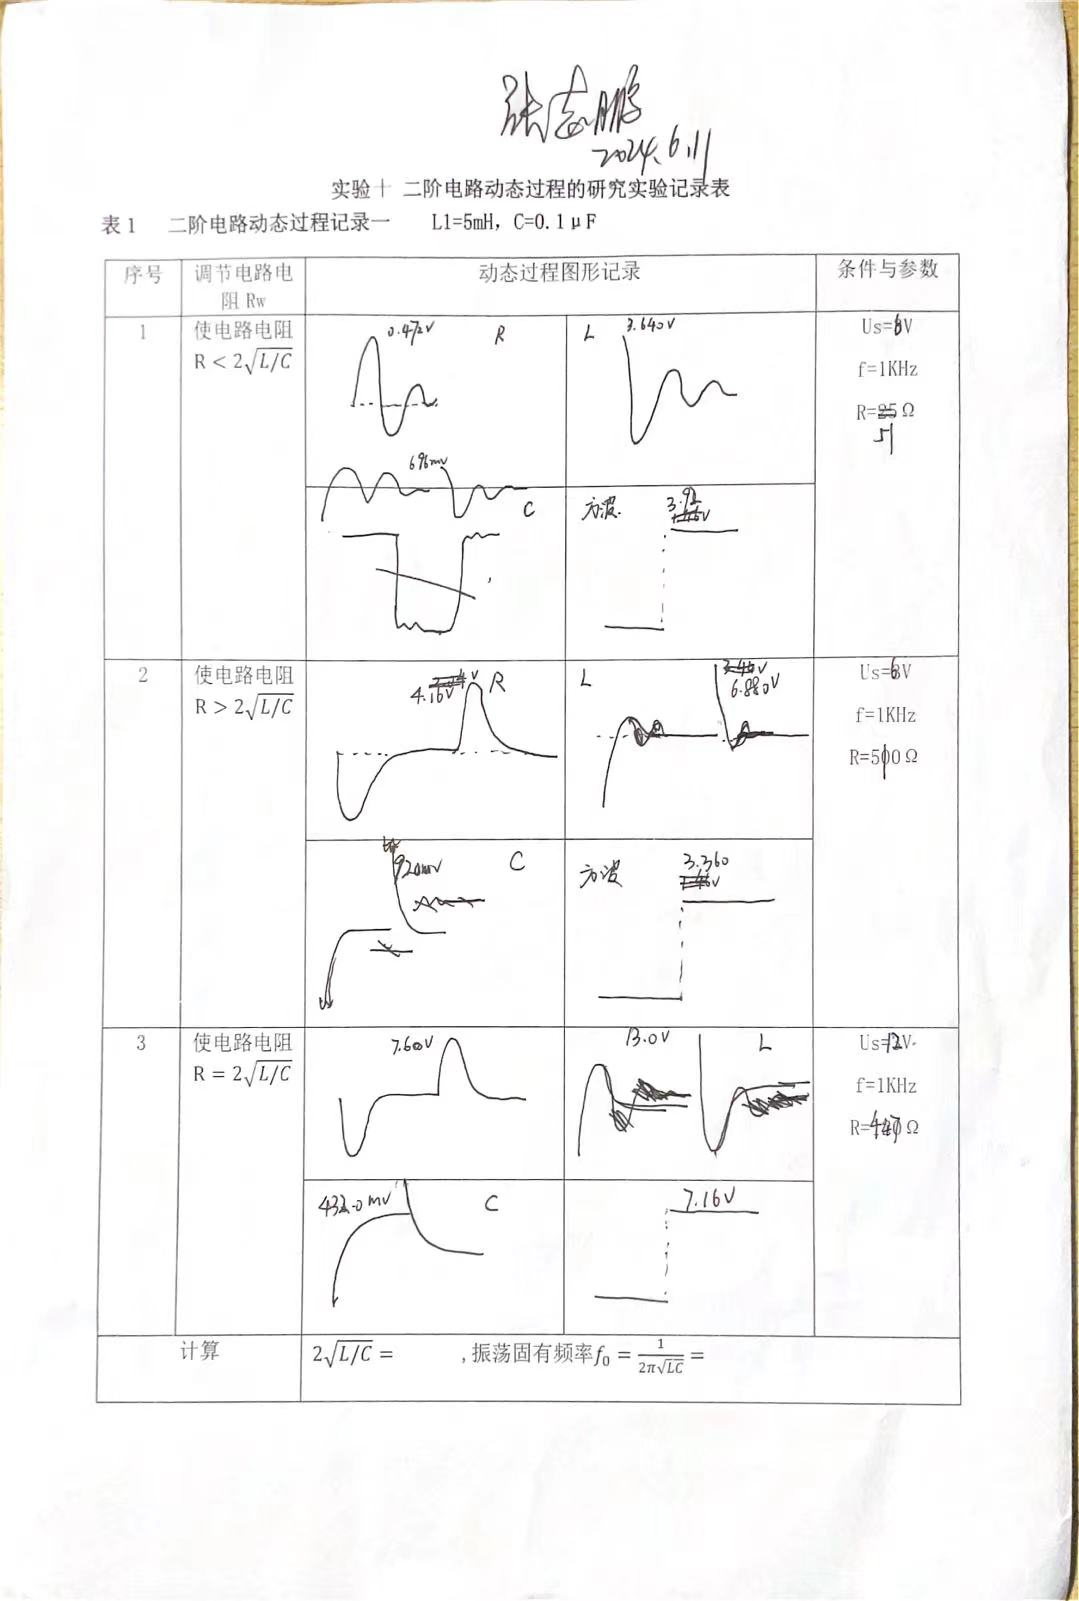
\includegraphics[width=0.7\textwidth]{data1.jpg}
    \end{center}
    \begin{center}    
        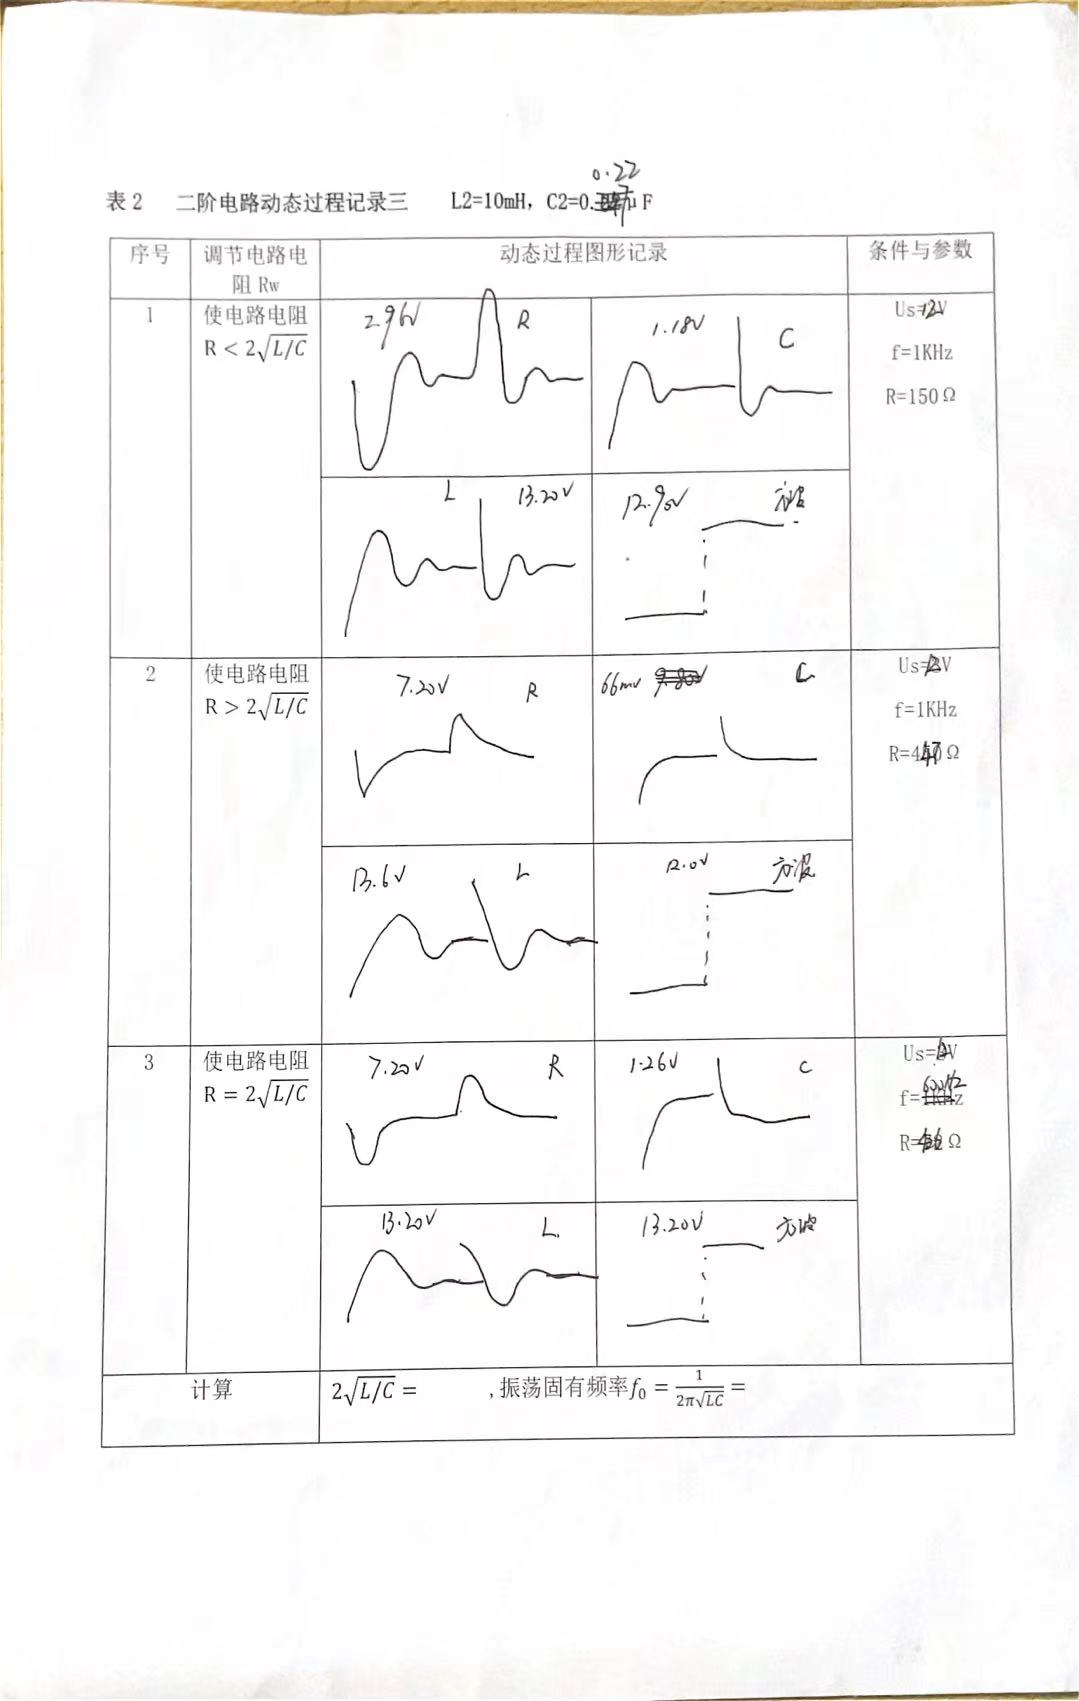
\includegraphics[width=0.7\textwidth]{data2.jpg}
    \end{center}
    \begin{center}    
        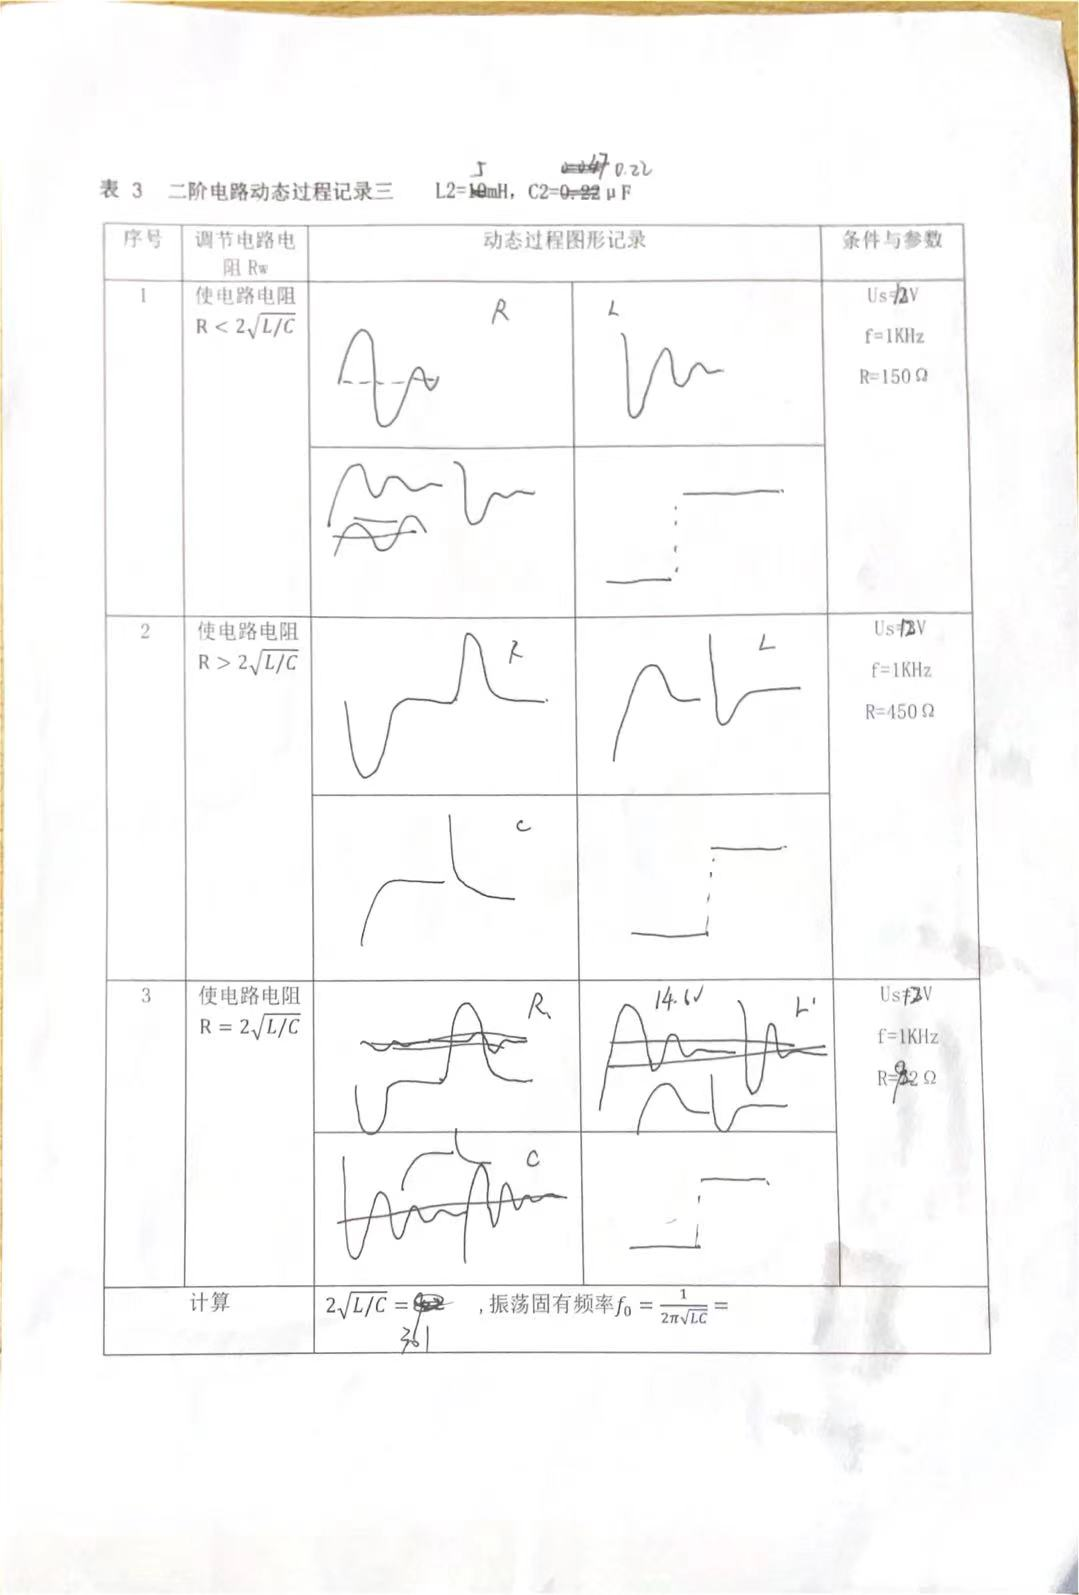
\includegraphics[width=0.7\textwidth]{data3.jpg}
    \end{center}
    \end{document}